% Shared body of the manuscript: one text, two renderings.
% jcheminf.tex adds double spacing and line numbers for the journal;
% main.tex renders the same text as a preprint. Edit the science in
% sections/, the order here, and never one rendering alone.
\begin{abstract}
The same compound measured against the same target in different laboratories receives different potency values, which limits how well any model can be scored against such labels. For 41 potency tasks (target $\times$ $K_i$ or $\mathrm{IC}_{50}$) from ChEMBL~37 we estimate that limit per task from 8{,}916 molecules reported in at least two source documents, and express model scores as a \emph{fraction of ceiling} $f$ (0: predicting the training mean; 1: reaching the estimated noise floor). The floors range from 0.31 to 0.92 pChEMBL units. After decontamination against MoleculeNet and TDC we benchmark ECFP-based models and frozen ChemBERTa-77M and MoLFormer-XL embeddings under four splits; the embeddings stay below ECFP on every one. The main result concerns the metric rather than the models. ECFP scores below the estimated floor on 16 of the 41 tasks under a random split, and $f$ rises with the noise it is meant to divide out ($\rho=+0.74$). The cause is document support: how much of a test molecule's own source document the model has already seen. Over 609{,}539 single-document test cases, RMSE falls from 1.07 pChEMBL with no same-document training molecule to 0.51 with a hundred or more, below the median floor of 0.54. With no support the random, scaffold and temporal splits give the same error, so their familiar ordering reflects document support rather than chemical difficulty. A constant per-document offset accounts for 57\% of the noise variance, too little to explain that gap. A document-grouped split puts every task back below the ceiling and removes the confounding ($\rho=+0.05$), while leaving the model ordering unchanged.

\textbf{Scientific Contribution.} We estimate the label-noise ceiling separately for each benchmark task from independent ChEMBL documents, instead of assuming one literature-wide noise level, and validate the estimate against held-out measurements. We show that scores at or beyond that ceiling are produced by document support, which also accounts for the apparent difficulty ordering of random, scaffold and temporal splits. We release a document-grouped split and code that computes the ceiling and the support distribution of any ChEMBL task.
\end{abstract}

\paragraph{Keywords} ChEMBL; label noise; noise ceiling; benchmarking; data splits; potency prediction; QSAR; reproducibility


% introduction.tex and results.tex already carry the heading the journal wants,
% so they are input ungrouped and only the files that follow them are demoted.
\section{Introduction}
Public potency data used to train and benchmark molecular machine-learning (ML) models come mostly from ChEMBL~\cite{zdrazil2024chembl}, a database manually curated from the literature. Potency is reported as an inhibition constant $K_i$ or as $\mathrm{IC}_{50}$, the concentration giving 50\% inhibition, and is usually converted to a pChEMBL value, $-\log_{10}$ of the molar value (pChEMBL 7 corresponds to 100\,nM). Each value comes from an \emph{assay} (an experimental protocol) reported in a \emph{document}, typically one publication; different documents usually mean different laboratories, protocols and reagents.

The same molecule measured against the same target in different documents often disagrees by more than 0.3 log units, and a sizeable fraction of pairs differ by more than one log unit~\cite{kalliokoski2013comparability,landrum2024combining}. Kramer et al.~\cite{kramer2012experimental} estimated the standard deviation of independent public $K_i$ measurements at 0.54 log units and the maximum achievable $R^2$ at about 0.81, and Brown et al.~\cite{brown2009healthy} argued that experimental error should set expectations for model performance. If two models differ in test error by less than this disagreement, a leaderboard gap says little about predictive quality. Later work bounds achievable performance by adding noise of an assumed or published size to labels~\cite{kolmar2021noise,crusius2025fitting}. Here we estimate the noise separately for each benchmark task, from molecules reported in at least two documents, and use it to put model scores on a common scale.

\paragraph{Splits.} How a dataset is divided into training and test molecules determines what a score means. A \emph{random} split puts close analogues on both sides and mainly rewards interpolation; a \emph{scaffold} split keeps all molecules sharing a Bemis--Murcko scaffold on one side, testing transfer to new chemotypes; a \emph{temporal} split trains on molecules first reported earlier and tests on later ones, mimicking prospective use. We report all three, and add a fourth, grouped by source document, for reasons that Section~\ref{sec:support} makes clear.

\paragraph{Contributions.}
\begin{enumerate}[nosep]
\item A per-task, test-set-specific use of a standard pooled replicate-variance estimator, in the spirit of earlier analyses of ChEMBL reproducibility~\cite{kramer2012experimental,kalliokoski2013comparability}, to obtain noise floors (RMSE and $R^2$), with bootstraps over molecules and over document pairs and sensitivity analyses for trimming, duplicated values, stereochemistry and assay selection (Section~\ref{sec:ceiling}).
\item A benchmark on 41 ChEMBL potency tasks after decontamination against MoleculeNet and TDC, comparing tuned ECFP models, frozen foundation-model embeddings, a D-MPNN and a fine-tuned chemical language model (Sections~\ref{sec:data}--\ref{sec:results}). Twenty-four of the tasks are targets added after the first version of this work, and serve as a replication set.
\item A test of whether replicates are independent, using the author lists and identifiers of all source documents: pairs that share an author agree markedly better than pairs that do not, so a floor built from all between-document pairs is conservative (Section~\ref{sec:provenance}).
\item The central negative result: the \emph{fraction of ceiling} does not put tasks with different noise on one scale, because it scales with that noise. The cause is document support --- how many molecules of a test molecule's own source document are in the training set. With no such support, random, scaffold and temporal splits are equally hard (Section~\ref{sec:support}). We propose and evaluate a document-grouped split as the remedy (Section~\ref{sec:docsplit}).
\end{enumerate}

\paragraph{Findings in brief.} The estimated floors range from 0.31 to 0.92 pChEMBL units, but for several tasks they rest on few document pairs and are uncertain. Frozen pretrained embeddings are consistently below ECFP, in agreement with recent large comparisons~\cite{praski2025benchmarking}; a three-task pilot that suggested the opposite under temporal shift did not replicate, first on 17 tasks and then on 24 further targets. The result we did not expect is that ECFP scores below the estimated floor on 16 of the 41 tasks under a random split, and that this tracks the estimated noise rather than any property of the models. Section~\ref{sec:support} traces it to document support and shows that the three splits do not differ in difficulty once support is held at zero, which makes the familiar random--scaffold--temporal ordering largely an artefact of how ChEMBL data are divided. We therefore recommend reading the noise ceiling as a leakage detector, and report a document-grouped split that removes the support (Section~\ref{sec:docsplit}).

\begin{jcgroup}
\section{Related work}
\paragraph{Noise in ChEMBL potency data.}
Kramer et al.~\cite{kramer2012experimental} analysed the reproducibility of independent $K_i$ measurements in ChEMBL; they report a standard deviation of 0.54 pK$_i$ units and a maximum achievable $R^2$ of about 0.81, and show that unit-transcription errors, undifferentiated stereoisomers and repeated citations of single measurements must be filtered. Kalliokoski et al.~\cite{kalliokoski2013comparability} found the standard deviation of mixed public $\mathrm{IC}_{50}$ data to be only about 25\% larger than that of $K_i$ data. Landrum and Riniker~\cite{landrum2024combining} quantified the disagreement between $\mathrm{IC}_{50}$ or $K_i$ values for the same compound--target pair from different ChEMBL assays: with minimal curation, about two thirds of pairs differ by more than 0.3 log units and about a quarter by more than one, and matching assay metadata reduces but does not remove the disagreement. Nelen et al.~\cite{nelen2025matched} show that matched-pair differences are more robust to inter-assay variability than absolute values. Schiebroek et al.~\cite{schiebroek2026balancing} evaluate curation strategies for bioactivity prediction. These works characterise the noise; we convert it into a per-task limit on achievable accuracy and rescore models against it.

\paragraph{Performance bounds from noise.}
Brown et al.~\cite{brown2009healthy} discussed how experimental error limits realistic model performance. Kolmar and Grulke~\cite{kolmar2021noise} studied how label noise limits the predictive performance of QSAR models. Crusius et al.~\cite{crusius2025fitting} derive realistic performance bounds by perturbing labels with noise of the size of the experimental error and report that models reach or exceed these bounds on several common datasets. The main difference to our work is the source of the noise estimate: they rely on an assumed or reported error magnitude, whereas we estimate it per task and test set from molecules reported in several documents, quantify its uncertainty, and use it to define a fraction-of-ceiling score. Their observation that models can reach or exceed noise-based bounds parallels our cases with $f>1$. Klamt et al.~\cite{klamt2026protac} attribute part of the generalisation gap in PROTAC activity prediction to inter-laboratory variance; their setting is a single domain with a classification metric.

\paragraph{Pretrained embeddings versus fingerprints.}
Praski et al.~\cite{praski2025benchmarking} compare 25 pretrained molecular embedding models on 25 datasets and find that nearly all perform no better than ECFP fingerprints. Guo and Ding~\cite{guo2026larger} and Kamuntavi\v{c}ius et al.~\cite{kamuntavicius2025admet} report similar strength of classical fingerprint models in activity and ADMET prediction. None of these accounts for label noise; our comparison expresses the gap relative to a measured floor and resolves it by split type.

\paragraph{Benchmark quality, leakage and evaluation protocols.}
Audits of widely used benchmarks report leakage, conflicting labels and redundancy~\cite{schuh2026auditing,huang2025litpcba}. Blevins and Quigley~\cite{blevins2025cleverhans} show that models can exploit signals of the chemist or publication rather than structure--activity relationships and propose author-disjoint splits; this is directly relevant to our observation that models can fall below a cross-document noise floor under random splits (Section~\ref{sec:results}). MoleculeACE~\cite{vantilborg2022exposing} benchmarks performance on activity cliffs. Ash et al.~\cite{ash2025practically} propose statistically grounded protocols for comparing methods; we add a noise-based reference point and empirical minimum detectable effects to that picture.

\paragraph{Models.}
We use ChemBERTa~\cite{chithrananda2020chemberta,ahmad2022chemberta2}, MoLFormer~\cite{ross2022molformer} and a directed message-passing neural network (D-MPNN)~\cite{yang2019analyzing}.

\end{jcgroup}

\section{Methods}
\begin{jcgroup}
\section{Data}\label{sec:data}
\paragraph{Source.}
Measurements were retrieved from the ChEMBL REST API on 10 October 2026; the API reported release ChEMBL~37 (released 1 May 2026)~\cite{zdrazil2024chembl}. We queried 59 single-protein targets (Appendix~\ref{app:repro}; identifiers checked against ChEMBL preferred names). Twenty-nine were chosen for the first version of this work; the further thirty were added afterwards by taking the human single-protein targets with the most binding $K_i$/$\mathrm{IC}_{50}$ activities carrying a pChEMBL value that were not already in the set (\texttt{scripts/}\allowbreak\texttt{13\_discover\_targets.py}; 242 of 5{,}869 targets have at least 1{,}500 such activities). We kept activities with standard type $K_i$ or $\mathrm{IC}_{50}$, relation `$=$', a pChEMBL value, binding assay type (B), no data-validity comment, no potential-duplicate flag, a document year, and an assay confidence score $\ge 8$. A score of 8 admits assays assigned to a homologous single protein, so assays on orthologues from other species may be included; we did not filter by organism or by mutant variant. Censored values (relations `$<$', `$>$') are dropped, which truncates the potency range at both ends.

\paragraph{Standardisation and aggregation.}
Structures were standardised with RDKit (largest fragment, neutralisation, canonical SMILES). Molecules are identified by the connectivity block of the InChIKey, so stereoisomers are merged (a stereo-aware sensitivity analysis is given in Section~\ref{sec:ceiling}). Within a document, values for a molecule are averaged, so that every remaining replicate is \emph{between} documents; note that one document can contain several assays (e.g.\ different enzyme variants or assay conditions), which this averaging mixes. A molecule's label is the mean over its documents; we also record the number of documents $n_i$ and the year of first report. A \emph{task} is a (target, measurement type) pair; $K_i$ and $\mathrm{IC}_{50}$ are never pooled. This gives 118 tasks.

\paragraph{Task selection.}
A task is kept if at least 100 molecules have values from $\ge2$ documents. Forty-one tasks pass after decontamination, 17 from the original 29 targets and 24 from the 30 added later (Table~\ref{tab:ceil}). They contain 1{,}000--9{,}567 molecules (median 4{,}778; 210{,}519 in total). Only 1.8--18.4\% of molecules per task (median 3.6\%) have replicates; after trimming (Section~\ref{sec:ceiling}) the floors are estimated from 8{,}916 replicated molecules. The 24 added tasks were analysed with the same pipeline and thresholds and serve as a replication set for the model comparison: they cover target classes the original set did not, among them a bromodomain, a deacetylase, two ion channels, a nuclear receptor and an isocitrate dehydrogenase.

\paragraph{Decontamination.}
We built a registry of molecules from 11 MoleculeNet and 40 TDC~\cite{huang2021tdc} datasets (202{,}019 unique structures) and removed, from the 41 tasks, molecules matching the registry by full InChIKey (5{,}393 molecules), additionally by InChIKey connectivity block (1{,}175), and near analogues with ECFP4 Tanimoto similarity $>0.8$ to any registry molecule (3{,}121): 9{,}689 of 220{,}208 molecules (4.4\%) in total. Replicated molecules were removed more often: 1{,}541 of 10{,}561 (15\%), since well-studied compounds are also the ones that appear in public benchmarks. Decontamination therefore changes the population from which the floor is estimated, and on the first 29 targets it reduced the number of tasks passing the threshold from 21 to 17. Polaris datasets could not be downloaded without authentication and are not included. Pretraining corpora of the foundation models (PubChem and ZINC subsets) were not screened; a filter removing documents published before the models' release left no task above the threshold and was therefore not applied. Unless stated otherwise, all results use the decontaminated data; the same models run on the uncleaned data are compared in Section~\ref{sec:results}.

\paragraph{Replicate statistics.}
An audit of the replicated pairs on the original 17 tasks before decontamination (\texttt{results/audit/}), in which pairs rather than molecules are trimmed, shows the following. The pooled between-document standard deviation depends strongly on how large disagreements are treated: its median over tasks is 0.65 log units without trimming, 0.57 when pairs differing by more than 3 log units are excluded and 0.45 when those differing by more than 2 are excluded. The disagreement is only weakly related to the time between the two publications (median Spearman $\rho=0.08$). Replicated molecules are not a random sample: on the decontaminated data they are on average 0.4--1.0 log units more potent than molecules reported only once in 7 of the 17 tasks.

\paragraph{Provenance of the replicates.} Whether two documents are genuinely independent, whether one re-publishes the other, and what assay conditions each used all bear on the floor, and none of them follows from the activity records alone. Section~\ref{sec:provenance} takes them up with document metadata: the first two can be measured, the third largely cannot. Species and mutant constructs we still do not check.

\section{Noise ceiling}\label{sec:ceiling}
\paragraph{Model.}
For molecule $i$ and document $j$ we write $y_{ij}=t_i+e_{ij}$ with $\E e_{ij}=0$ and $\Var e_{ij}=s^2$, where $t_i$ is the value the molecule would have in an idealised common assay and $e_{ij}$ collects all between-document variation (laboratory, protocol, reagents, curation and recording errors). Values within a document are averaged first. With $n_i$ documents for molecule $i$ and mean $\bar y_i$, the pooled within-molecule variance over molecules with $n_i\ge 2$ is
\begin{equation}
\hat s^2=\frac{\sum_i\sum_{j}(y_{ij}-\bar y_i)^2}{\sum_i (n_i-1)} .
\end{equation}
This is the standard pooled estimator used in earlier analyses of public potency data~\cite{kramer2012experimental,kalliokoski2013comparability}. Molecules whose document values span more than 3 pChEMBL units are excluded from the estimate as likely unit or recording errors (they remain in the training and test sets with their averaged labels).

\paragraph{Floors.}
The label of molecule $i$ is $\bar y_i$, whose noise variance is $s^2/n_i$. For a set of test molecules,
\begin{equation}
\mathrm{RMSE}_{\mathrm{floor}}=\sqrt{\hat s^2\,\overline{(1/n_i)}},\qquad
R^2_{\max}=1-\frac{\hat s^2\,\overline{(1/n_i)}}{\Var(y)},
\end{equation}
where the average of $1/n_i$ is taken over the test molecules of each split. If $e_{ij}$ is independent of everything a model can learn, a model that predicted every $t_i$ exactly would still have an expected test RMSE of $\mathrm{RMSE}_{\mathrm{floor}}$, and no model can be below it in expectation~\cite{kolmar2021noise}.

\paragraph{Fraction of ceiling.}
\begin{equation}
f=\frac{\mathrm{RMSE}_{\text{mean}}-\mathrm{RMSE}_{\text{model}}}{\mathrm{RMSE}_{\text{mean}}-\mathrm{RMSE}_{\mathrm{floor}}},
\end{equation}
where $\mathrm{RMSE}_{\text{mean}}$ is the RMSE of predicting the training-set mean on the same test set. Two words for one thing: the \emph{floor} is the lowest RMSE the labels allow, and the \emph{ceiling} is the same bound seen as the highest attainable score, $f=1$. A model that scores better than the labels should allow is thus said to fall below the floor and to pass the ceiling interchangeably. $f=0$ means no better than the mean, $f=1$ means at the noise floor, $f<0$ worse than the mean. Values $f>1$ mean that the floor overstates the noise that matters for this test set, or that there is leakage; they must be investigated rather than reported as success. The aim of $f$ is to put tasks with different noise levels on one scale, but it inherits the uncertainty of the floor and amplifies it when the headroom $\mathrm{RMSE}_{\text{mean}}-\mathrm{RMSE}_{\mathrm{floor}}$ is small, which is the case for the tasks with the largest floors. We therefore report medians and per-task values next to means, and the range of mean $f$ when the floor is computed at the ends of the confidence interval of $\hat s$. That is not the only problem with $f$, and not the worst one: Section~\ref{sec:support} shows that it is also systematically confounded with the noise it is meant to divide out, for reasons that have nothing to do with the uncertainty of the floor. A reader should take the definition here as the quantity we measure, not as a scale that can be compared across tasks without further care.

\paragraph{Uncertainty.}
We report two bootstraps (1{,}000 resamples, percentile 95\% intervals). The first resamples molecules; it treats every replicated molecule as independent. The second resamples \emph{document pairs}: a systematic offset between two documents is shared by all molecules they have in common, so the document pair, not the molecule, is the independent unit. For the second we use the pairwise form $\hat s^2=\sum \Delta^2/2 \,/\, N_{\text{pairs}}$ over all between-document differences $\Delta$, which equals the pooled estimator when every molecule has two documents. We also report, per task, the number of distinct document pairs and the share of molecule pairs contributed by the most frequent one.

\paragraph{Sensitivity analyses.}
(i) Trimming threshold ($\infty$, 3, 2, 1 pChEMBL units). Lower thresholds remove more genuine disagreement and make the floor smaller, so models look further from it; a higher threshold keeps gross recording errors and makes the floor larger. Over the first 17 tasks the median $\hat s$ is 0.61 without trimming, 0.53 with the default threshold of 3, 0.41 with 2 and 0.29 with 1 log unit (over all 41 the default-threshold median is 0.54); Table~\ref{tab:robust} reports every task. The 3-unit rule removes at most 2.5\% of replicated molecules per task, except for CHEMBL206 ($\mathrm{IC}_{50}$, 19\%). (ii) Requiring $\ge3$ documents leaves a median of only 15 replicated molecules per task (minimum 3) and is not used. (iii) Identical values reported by different documents, which are likely re-publications of one measurement~\cite{kramer2012experimental}, counted once. (iv) Molecules defined by the full stereo-aware SMILES instead of the InChIKey connectivity block. (v) Only the largest assay of each document. Results are in Table~\ref{tab:robust}.

\paragraph{Validation.} On one synthetic data set the estimator recovers the true value ($\hat s=0.42$ for $s=0.40$). This is a sanity check, not a study of bias and coverage under heteroscedastic noise or document-level offsets, which remains to be done.

\section{Benchmark}\label{sec:bench}
\paragraph{Models.}
\begin{itemize}[nosep]
\item \textbf{ECFP models.} Count-based Morgan fingerprints (radius 2, 2{,}048 bits, RDKit) with histogram gradient boosting (GBM), random forest (RF, 300 trees) or a multilayer perceptron (MLP), all from scikit-learn. ECFP+GBM is the reference model for paired comparisons.
\item \textbf{Frozen embeddings.} ChemBERTa-77M-MLM~\cite{ahmad2022chemberta2} (DeepChem/ChemBERTa-77M-MLM) and MoLFormer-XL trained on 10\% of its corpus~\cite{ross2022molformer} (ibm-research/MoLFormer-XL-both-10pct). Embeddings are the attention-masked mean of the last hidden layer for the canonical SMILES (maximum 256 tokens), with a GBM head. Hugging Face revisions are pinned: ChemBERTa \texttt{ed8a537}, MoLFormer \texttt{7b12d94} (March 2024; the latest revision requires a newer \texttt{transformers} release).
\item \textbf{D-MPNN.} A directed message-passing network~\cite{yang2019analyzing} implemented in PyTorch (mean pooling, early stopping on 10\% of the training set, at most 60 epochs, patience 10). Run on five tasks with three seeds because of its cost on CPU.
\item \textbf{Fine-tuned ChemBERTa.} ChemBERTa-77M-MLM fine-tuned end to end with a linear head on the mean-pooled representation (AdamW, learning rate for the encoder chosen from $\{2\cdot10^{-5},10^{-4}\}$ on an inner validation split, $10^{-3}$ for the head, batch size 32, early stopping with patience 5, at most 40 epochs, standardised targets). Run on the same five tasks with three seeds (five on one task).
\end{itemize}

\paragraph{Hyperparameters.}
All ECFP models, embedding heads and the D-MPNN receive the same budget: three configurations sampled from a fixed grid (Appendix~\ref{app:repro}), selected by RMSE on a random 20\% of the training set, then refitted on the full training set. The inner validation split is random for all outer splits, i.e.\ it does not mimic the scaffold or temporal shift. This is a small budget; it is equal across these families. The fine-tuned ChemBERTa has a different budget (two learning rates, 10\% validation, no refit). ECFP+MLP (standardised count fingerprints, scikit-learn MLP) performs poorly, below the training mean on temporal splits; it should be read as an untuned baseline, not as representative of neural networks on fingerprints.

\paragraph{Splits and seeds.}
Test sets are 20\% of the molecules. Random split: uniform at random. Scaffold split: Bemis--Murcko scaffold groups in random order are assigned to the test set while they fit, so large scaffold groups stay in training. Temporal split~\cite{sheridan2013timesplit}: the 20\% of molecules first reported most recently form the test set (deterministic; the test sets start between 2010 and 2022 depending on task, median 2019). Molecules first reported in the cut-off year are divided between training and test by file order, and training labels average all documents of a molecule, including documents published after the cut-off; the split is therefore slightly optimistic. Document split: whole source documents in random order are assigned to the test set while they fit, so that a test molecule shares no document with any training molecule, by the same construction as the scaffold split. We add it for the reason given in Section~\ref{sec:support} and evaluate it in Section~\ref{sec:docsplit}; a reader following the paper in order can treat it as a fourth split alongside the other three. Random, scaffold and document splits use five seeds; for the temporal split the seeds affect only model training.

\paragraph{Evaluation.}
For each task, split, seed and model we compute RMSE, $R^2$ and $f$ on the test set, average over seeds, and then over tasks. Uncertainty for averages is a bootstrap over test molecules (300 resamples). Comparisons with ECFP+GBM are paired by task: we report the mean difference in $f$, the number of tasks on which the model is better, and a Wilcoxon signed-rank test over the 41 tasks with Holm correction over all model--split comparisons. The test treats tasks as independent, which is approximate: CHEMBL237 appears with both $K_i$ and $\mathrm{IC}_{50}$, and related receptors (D$_2$/D$_3$, $\mu$/$\kappa$ opioid) share ligands. Models run on a subset of tasks are compared only on that subset and without tests.

\paragraph{Software and tooling.} The pipeline is written in Python; the versions of every library that affects a result are pinned in \texttt{requirements-lock.txt} in the repository. Parts of the analysis code and of the manuscript text were drafted with the assistance of a large language model (Anthropic Claude) working under the authors' direction. No result in this article was taken from that model: every number reported is produced by the released scripts from the released data, and was checked by the authors against an independent reimplementation.

\end{jcgroup}

% Generated by scripts/make_paper_tables.py -- do not edit by hand.
\section{Results}\label{sec:results}
Unless noted, results are averages over the 41 decontaminated tasks and five seeds.

\paragraph{Noise floors.} Table~\ref{tab:ceil} lists the estimates. $\mathrm{RMSE}_{\mathrm{floor}}$ ranges from 0.31 to 0.92 pChEMBL units and $R^2_{\max}$ from 0.30 to 0.96. The median $\hat s$ is 0.54 for $K_i$ tasks and 0.55 for $\mathrm{IC}_{50}$ tasks, of the same order as earlier ChEMBL-wide estimates for $K_i$ (0.54)~\cite{kramer2012experimental} and the reported 25\% larger spread of $\mathrm{IC}_{50}$ data~\cite{kalliokoski2013comparability}; in our set the measurement type is confounded with target class ($K_i$ tasks are mostly GPCRs, $\mathrm{IC}_{50}$ tasks mostly kinases), so we do not attribute the difference to the measurement type. Replicates are often concentrated in few document pairs: CHEMBL237\_IC50 rests on 7 document pairs, one of which contributes 79\% of molecule pairs. Accordingly, the bootstrap over document pairs gives intervals more than 20\% wider than the bootstrap over molecules for 30 of 41 tasks, and 4 and 5 times as wide for CHEMBL237\_IC50 and CHEMBL2971\_IC50 (for the latter, 0.53--1.15); it is narrower only for tasks with many document pairs. Table~\ref{tab:robust} shows the sensitivity to curation: counting identical values from different documents once raises $\hat s$ by up to 0.20 (CHEMBL237\_Ki), and a stereo-aware molecule definition changes it by more than 0.05 for 17 tasks. These are the uncertainties of the reference point against which all models below are scored.

\paragraph{Fraction of ceiling.} Table~\ref{tab:frac} gives mean $f$ by model and split. ECFP+RF is the best model on every split. On random splits its mean $f$ is 1.04, but the median is 0.93, the mean without the tasks where it exceeds 1 is 0.83, and computing the floor at the ends of the confidence interval of $\hat s$ moves the mean between 0.89 and 1.33. On scaffold and temporal splits the means are 0.87 and 0.42 (medians 0.74 and 0.35), and 0.38 on the document-grouped split of Section~\ref{sec:docsplit}. The apparent ease of random splits is not a property of the chemistry: Section~\ref{sec:support} shows that it comes from training molecules drawn from the test molecule's own source document, and once documents are kept apart the best model reaches about 38\% of the ceiling rather than passing it.

\paragraph{ECFP versus frozen embeddings.} Frozen ChemBERTa-77M and MoLFormer-XL-10\% embeddings with a GBM head are below ECFP+GBM on every split (Table~\ref{tab:paired}, Figure~\ref{fig:paired}): by 0.19--0.25 in $f$ on random and scaffold splits, where they are worse on all 41 tasks, and by 0.07--0.08 on temporal splits, where they are better on only 9--12 of 41 tasks (Holm-adjusted $p\le0.002$ in all cases). ECFP+RF is slightly better than ECFP+GBM (0.02--0.04 in $f$; better on 30--32 of 41 tasks). In a three-task pilot (CHEMBL237\_IC50, CHEMBL206\_IC50, CHEMBL204\_Ki) frozen embeddings had appeared better than ECFP on temporal splits; on 41 tasks this did not hold. The conclusion concerns two small frozen models with a tree-based head, not pretrained models in general.

\paragraph{D-MPNN and fine-tuning.} Table~\ref{tab:subset} compares all models on the 5 tasks where the D-MPNN and fine-tuned ChemBERTa were run. On random and scaffold splits neither reaches ECFP, and fine-tuning does not improve on the frozen embedding. On temporal splits the fine-tuned model has the highest mean (0.31 versus 0.28 for ECFP+RF), but this comes from a single task, CHEMBL237\_IC50 (0.48 versus 0.08); on the other 4 tasks the means are 0.27 and 0.33. With 5 tasks we do not test these differences.

\paragraph{Models below the noise floor.} On 25 task--split combinations ECFP+RF scores $f>1$, i.e.\ its test RMSE is below the estimated floor (Figure~\ref{fig:floor}), 17 of them on random splits and none on the document-grouped split. If between-document noise were independent of what a model can learn, this would be impossible in expectation~\cite{kolmar2021noise}; models reaching or exceeding noise-based bounds were also reported by Crusius et al.~\cite{crusius2025fitting}. Section~\ref{sec:support} shows that these cases are not scattered anomalies: $f$ rises with the estimated noise it is meant to divide out, and what carries a model past the floor is how many training molecules come from the test molecule's own source document. Models are known to exploit publication-level signals in ChEMBL~\cite{blevins2025cleverhans}. Floor mis-estimation contributes as well for individual tasks --- for CHEMBL2971\_IC50 the interval over document pairs is very wide (0.53--1.15), and two of its document pairs differ by a nearly constant 2.4 and 3.0 log units (standard deviations 0.41 and 0.13 over 29 and 26 shared molecules), which suggests unit errors that the 3-unit trimming does not remove. Under the document-grouped split of Section~\ref{sec:docsplit} no task exceeds the floor. In either case $f>1$ signals a problem with the split or the floor, not accuracy beyond the measurement limit.

\paragraph{Minimum detectable effect.} The median single-test-set MDE for a paired comparison with ECFP+GBM is 0.047, 0.048 and 0.054 in $f$ for ECFP+RF on random, scaffold and temporal splits, and about 0.09 for the embedding models, whose errors are less correlated with the baseline. These values assume independent test molecules and are therefore optimistic. The ECFP+RF advantage is below the MDE of a single test set and is detectable only when pooled over tasks, while the embedding gaps on random and scaffold splits are two to three times the MDE.

\begin{table}[ht]\centering\footnotesize\setlength{\tabcolsep}{4pt}\caption{Noise floors per task (decontaminated data). $n_{\text{rep}}$: replicated molecules after trimming; doc.\ pairs: distinct pairs of documents among the replicates; top \%: share of molecule pairs from the most frequent document pair. 95\% intervals for $\hat s$ from a bootstrap over molecules and over document pairs (1{,}000 resamples); the latter is for the pairwise form of the estimator, which differs slightly from $\hat s$ when molecules have more than two documents. $\mathrm{RMSE}_{\mathrm{floor}}$ and $R^2_{\max}$ over all molecules of the task.}\label{tab:ceil}
\begin{tabular}{lrrrccccc}\toprule Task & $n_{\text{rep}}$ & doc.\ pairs & top \% & $\hat s$ & CI molecules & CI doc.\ pairs & $\mathrm{RMSE}_{\mathrm{floor}}$ & $R^2_{\max}$\\\midrule
CHEMBL1163125\_IC50 & 224 & 270 & 17 & 0.54 & [0.50, 0.58] & [0.50, 0.63] & 0.53 & 0.79\\
CHEMBL1741186\_IC50 & 210 & 131 & 9 & 0.50 & [0.45, 0.56] & [0.43, 0.60] & 0.50 & 0.71\\
CHEMBL1865\_IC50 & 162 & 198 & 7 & 0.66 & [0.57, 0.75] & [0.57, 0.83] & 0.65 & 0.60\\
CHEMBL2007625\_IC50 & 522 & 139 & 23 & 0.46 & [0.42, 0.49] & [0.44, 0.60] & 0.44 & 0.75\\
CHEMBL2039\_IC50 & 107 & 84 & 7 & 0.78 & [0.63, 0.90] & [0.60, 0.98] & 0.77 & 0.58\\
CHEMBL203\_IC50 & 396 & 432 & 17 & 0.66 & [0.61, 0.70] & [0.61, 0.71] & 0.65 & 0.75\\
CHEMBL2041\_IC50 & 369 & 107 & 60 & 0.59 & [0.56, 0.62] & [0.50, 0.66] & 0.58 & 0.65\\
CHEMBL204\_Ki & 133 & 108 & 8 & 0.31 & [0.19, 0.43] & [0.24, 0.44] & 0.31 & 0.96\\
CHEMBL205\_Ki & 156 & 117 & 6 & 0.70 & [0.62, 0.78] & [0.63, 0.82] & 0.70 & 0.62\\
CHEMBL206\_IC50 & 132 & 103 & 13 & 0.53 & [0.42, 0.63] & [0.43, 0.70] & 0.52 & 0.85\\
CHEMBL2148\_IC50 & 187 & 169 & 15 & 0.74 & [0.65, 0.83] & [0.62, 0.93] & 0.73 & 0.67\\
CHEMBL214\_Ki & 147 & 79 & 11 & 0.49 & [0.41, 0.57] & [0.43, 0.64] & 0.49 & 0.82\\
CHEMBL217\_Ki & 185 & 157 & 7 & 0.44 & [0.38, 0.49] & [0.41, 0.53] & 0.44 & 0.80\\
CHEMBL220\_IC50 & 210 & 262 & 5 & 0.53 & [0.44, 0.61] & [0.50, 0.65] & 0.52 & 0.84\\
CHEMBL233\_Ki & 155 & 404 & 2 & 0.55 & [0.44, 0.63] & [0.58, 0.69] & 0.54 & 0.81\\
CHEMBL234\_Ki & 127 & 176 & 5 & 0.42 & [0.35, 0.49] & [0.38, 0.51] & 0.42 & 0.89\\
CHEMBL237\_IC50 & 111 & 7 & 79 & 0.69 & [0.66, 0.74] & [0.51, 0.83] & 0.67 & 0.63\\
CHEMBL237\_Ki & 131 & 105 & 7 & 0.54 & [0.42, 0.64] & [0.46, 0.69] & 0.53 & 0.84\\
CHEMBL251\_Ki & 106 & 97 & 9 & 0.44 & [0.36, 0.52] & [0.36, 0.51] & 0.44 & 0.86\\
CHEMBL261\_Ki & 115 & 81 & 7 & 0.71 & [0.58, 0.82] & [0.60, 0.89] & 0.71 & 0.53\\
CHEMBL279\_IC50 & 229 & 312 & 14 & 0.70 & [0.64, 0.77] & [0.59, 0.80] & 0.70 & 0.61\\
CHEMBL2815\_IC50 & 135 & 378 & 6 & 0.93 & [0.83, 1.04] & [0.66, 0.98] & 0.92 & 0.30\\
CHEMBL2835\_IC50 & 440 & 139 & 23 & 0.55 & [0.51, 0.59] & [0.38, 0.67] & 0.54 & 0.81\\
CHEMBL2971\_IC50 & 526 & 153 & 35 & 0.80 & [0.74, 0.86] & [0.53, 1.15] & 0.79 & 0.56\\
CHEMBL2998\_IC50 & 125 & 22 & 16 & 0.39 & [0.30, 0.47] & [0.37, 0.44] & 0.38 & 0.74\\
CHEMBL3130\_IC50 & 304 & 145 & 20 & 0.52 & [0.47, 0.58] & [0.44, 0.68] & 0.52 & 0.81\\
CHEMBL325\_IC50 & 218 & 264 & 3 & 0.67 & [0.59, 0.75] & [0.57, 0.78] & 0.67 & 0.63\\
CHEMBL3553\_IC50 & 175 & 106 & 20 & 0.60 & [0.52, 0.67] & [0.56, 0.74] & 0.59 & 0.66\\
CHEMBL3778\_IC50 & 144 & 75 & 10 & 0.65 & [0.55, 0.75] & [0.48, 0.77] & 0.65 & 0.65\\
CHEMBL4005\_IC50 & 104 & 73 & 16 & 0.39 & [0.29, 0.50] & [0.32, 0.59] & 0.39 & 0.88\\
CHEMBL4040\_IC50 & 129 & 36 & 34 & 0.70 & [0.59, 0.80] & [0.49, 1.05] & 0.70 & 0.65\\
CHEMBL4296\_IC50 & 148 & 69 & 13 & 0.46 & [0.40, 0.52] & [0.40, 0.55] & 0.46 & 0.79\\
CHEMBL4792\_Ki & 358 & 30 & 74 & 0.84 & [0.79, 0.89] & [0.41, 0.90] & 0.80 & 0.51\\
CHEMBL4805\_IC50 & 251 & 45 & 45 & 0.54 & [0.45, 0.64] & [0.23, 0.95] & 0.53 & 0.57\\
CHEMBL4822\_IC50 & 308 & 130 & 14 & 0.50 & [0.43, 0.56] & [0.44, 0.60] & 0.49 & 0.84\\
CHEMBL5113\_Ki & 357 & 29 & 75 & 0.84 & [0.79, 0.88] & [0.36, 0.89] & 0.80 & 0.42\\
CHEMBL5145\_IC50 & 128 & 63 & 31 & 0.48 & [0.38, 0.57] & [0.34, 0.67] & 0.47 & 0.85\\
CHEMBL5251\_IC50 & 528 & 243 & 10 & 0.63 & [0.58, 0.68] & [0.55, 0.71] & 0.62 & 0.71\\
CHEMBL5804\_IC50 & 116 & 6 & 92 & 0.31 & [0.27, 0.36] & [0.29, 0.45] & 0.31 & 0.80\\
CHEMBL5805\_IC50 & 147 & 6 & 85 & 0.54 & [0.49, 0.60] & [0.18, 0.58] & 0.54 & 0.62\\
CHEMBL5936\_IC50 & 161 & 7 & 85 & 0.49 & [0.43, 0.54] & [0.22, 0.51] & 0.48 & 0.83\\
\bottomrule\end{tabular}\end{table}

\begin{table}[ht]\centering\small\setlength{\tabcolsep}{4pt}\caption{Sensitivity of $\hat s$ to curation choices. ident.\ \%: share of between-document pairs with identical values; no dup.: identical values from different documents counted once; stereo: molecules defined by stereo-aware SMILES; one assay: only the largest assay of each document; multi-assay \%: molecule--document pairs with values from more than one assay.}\label{tab:robust}
\begin{tabular}{lcccccc}\toprule Task & $\hat s$ & ident.\ \% & no dup. & stereo & one assay & multi-assay \%\\\midrule
CHEMBL203\_IC50 & 0.66 & 5 & 0.68 & 0.66 & 0.65 & 26\\
CHEMBL204\_Ki & 0.31 & 34 & 0.38 & 0.37 & 0.34 & 1\\
CHEMBL205\_Ki & 0.70 & 14 & 0.76 & 0.72 & 0.69 & 0\\
CHEMBL206\_IC50 & 0.53 & 15 & 0.58 & 0.54 & 0.50 & 32\\
CHEMBL214\_Ki & 0.49 & 12 & 0.52 & 0.50 & 0.51 & 1\\
CHEMBL217\_Ki & 0.44 & 10 & 0.46 & 0.50 & 0.43 & 11\\
CHEMBL233\_Ki & 0.55 & 16 & 0.67 & 0.46 & 0.55 & 0\\
CHEMBL234\_Ki & 0.42 & 6 & 0.44 & 0.45 & 0.43 & 10\\
CHEMBL237\_IC50 & 0.69 & 6 & 0.72 & 0.70 & 0.69 & 2\\
CHEMBL237\_Ki & 0.54 & 33 & 0.67 & 0.46 & 0.58 & 1\\
CHEMBL251\_Ki & 0.44 & 9 & 0.47 & 0.43 & 0.48 & 1\\
CHEMBL279\_IC50 & 0.70 & 5 & 0.74 & 0.69 & 0.68 & 11\\
CHEMBL2971\_IC50 & 0.80 & 7 & 0.82 & 0.85 & 0.80 & 5\\
CHEMBL325\_IC50 & 0.67 & 3 & 0.68 & 0.67 & 0.55 & 1\\
CHEMBL4005\_IC50 & 0.39 & 20 & 0.45 & 0.45 & 0.38 & 4\\
CHEMBL4822\_IC50 & 0.50 & 21 & 0.56 & 0.62 & 0.51 & 15\\
CHEMBL5145\_IC50 & 0.48 & 1 & 0.48 & 0.47 & 0.44 & 18\\
CHEMBL1163125\_IC50 & 0.54 & 7 & 0.57 & 0.57 & 0.59 & 23\\
CHEMBL1741186\_IC50 & 0.50 & 9 & 0.53 & 0.60 & 0.50 & 18\\
CHEMBL1865\_IC50 & 0.66 & 8 & 0.70 & 0.70 & 0.54 & 6\\
CHEMBL2007625\_IC50 & 0.46 & 4 & 0.47 & 0.55 & 0.51 & 31\\
CHEMBL2039\_IC50 & 0.78 & 13 & 0.84 & 0.82 & 0.75 & 3\\
CHEMBL2041\_IC50 & 0.59 & 7 & 0.62 & 0.62 & 0.59 & 58\\
CHEMBL2148\_IC50 & 0.74 & 15 & 0.83 & 0.80 & 0.76 & 6\\
CHEMBL220\_IC50 & 0.53 & 21 & 0.62 & 0.52 & 0.51 & 3\\
CHEMBL261\_Ki & 0.71 & 16 & 0.79 & 0.79 & 0.73 & 0\\
CHEMBL2815\_IC50 & 0.93 & 12 & 1.08 & 1.07 & 0.96 & 24\\
CHEMBL2835\_IC50 & 0.55 & 12 & 0.59 & 0.63 & 0.55 & 3\\
CHEMBL2998\_IC50 & 0.39 & 13 & 0.39 & 0.53 & 0.38 & 0\\
CHEMBL3130\_IC50 & 0.52 & 10 & 0.54 & 0.51 & 0.46 & 5\\
CHEMBL3553\_IC50 & 0.60 & 21 & 0.69 & 0.73 & 0.59 & 4\\
CHEMBL3778\_IC50 & 0.65 & 16 & 0.72 & 0.68 & 0.73 & 4\\
CHEMBL4040\_IC50 & 0.70 & 35 & 0.90 & 1.16 & 0.72 & 4\\
CHEMBL4296\_IC50 & 0.46 & 7 & 0.47 & 0.49 & 0.43 & 11\\
CHEMBL4792\_Ki & 0.84 & 2 & 0.85 & 0.88 & 0.84 & 0\\
CHEMBL4805\_IC50 & 0.54 & 1 & 0.55 & 0.58 & 0.54 & 6\\
CHEMBL5113\_Ki & 0.84 & 2 & 0.85 & 0.86 & 0.84 & 0\\
CHEMBL5251\_IC50 & 0.63 & 15 & 0.70 & 0.75 & 0.61 & 8\\
CHEMBL5804\_IC50 & 0.31 & 1 & 0.32 & 0.34 & 0.31 & 0\\
CHEMBL5805\_IC50 & 0.54 & 2 & 0.55 & 0.55 & 0.55 & 1\\
CHEMBL5936\_IC50 & 0.49 & 2 & 0.49 & 0.51 & 0.49 & 0\\
\bottomrule\end{tabular}\end{table}

\begin{figure}[ht]\centering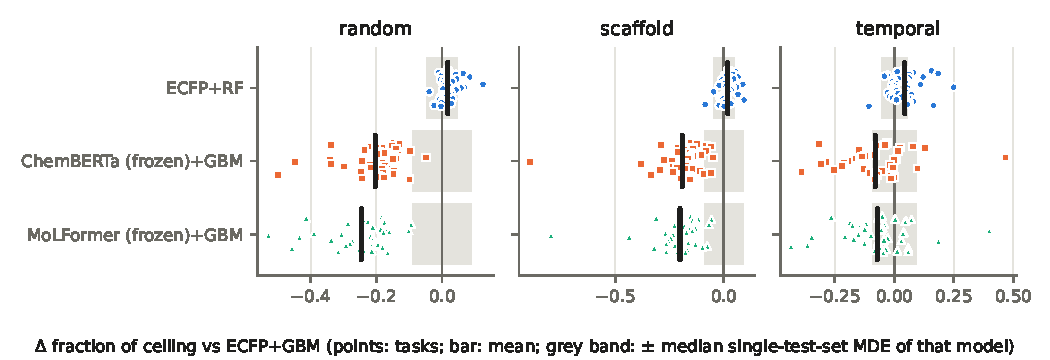
\includegraphics[width=\linewidth]{figures/paired_diff.pdf}
\caption{Per-task difference in fraction of ceiling relative to ECFP+GBM (points: tasks; bar: mean over tasks; grey band: $\pm$ median single-test-set MDE of each model).}\label{fig:paired}\end{figure}

\begin{figure}[ht]\centering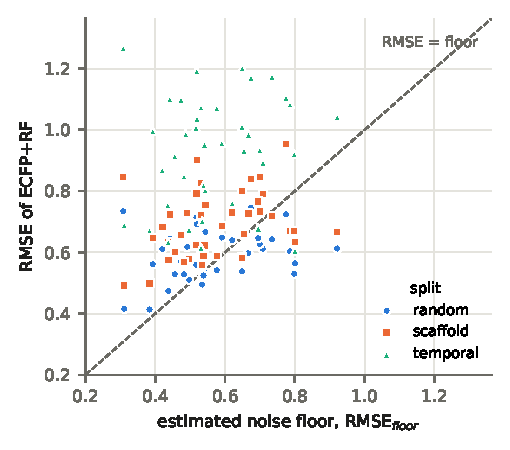
\includegraphics[width=0.5\linewidth]{figures/floor_vs_rmse.pdf}
\caption{Estimated noise floor versus test RMSE of ECFP+RF per task and split. Points below the dashed line have RMSE below the estimated floor ($f>1$).}\label{fig:floor}\end{figure}

\begin{table}[ht]\centering\small\setlength{\tabcolsep}{4pt}\caption{Mean fraction of ceiling $f$ over tasks ($n$ = number of tasks), decontaminated data. Models with $n<41$ were run on a subset of tasks and are not comparable with the rest (see Table~\ref{tab:subset}).}\label{tab:frac}
\begin{tabular}{lccccc}\toprule Model & $n$ & Random & Scaffold & Temporal & Document\\\midrule
ECFP+GBM & 41 & 1.02 & 0.85 & 0.37 & 0.34\\
ECFP+RF & 41 & 1.04 & 0.87 & 0.42 & 0.38\\
ECFP+MLP & 41 & 0.51 & 0.08 & -1.01 & -0.93\\
ChemBERTa-77M (frozen)+GBM & 41 & 0.82 & 0.66 & 0.29 & 0.28\\
MoLFormer-XL-10\% (frozen)+GBM & 41 & 0.78 & 0.65 & 0.30 & 0.30\\
D-MPNN & 5 & 0.63 & 0.54 & 0.27 & --\\
ChemBERTa-77M (fine-tuned) & 5 & 0.60 & 0.49 & 0.31 & --\\
\bottomrule\end{tabular}\end{table}

\begin{table}[ht]\centering\small\setlength{\tabcolsep}{4pt}\caption{Paired difference in $f$ versus ECFP+GBM over 41 tasks (positive = better than ECFP+GBM); Wilcoxon signed-rank test, Holm-adjusted $p$.}\label{tab:paired}
\begin{tabular}{llccc}\toprule Model & Split & mean diff. & better on & $p_{\text{Holm}}$\\\midrule
ECFP+RF & random & +0.018 & 30/41 & 0.001\\
ECFP+RF & scaffold & +0.017 & 31/41 & 0.002\\
ECFP+RF & temporal & +0.043 & 31/41 & $<$0.001\\
ECFP+RF & document & +0.041 & 32/41 & $<$0.001\\
ECFP+MLP & random & -0.514 & 0/41 & $<$0.001\\
ECFP+MLP & scaffold & -0.777 & 0/41 & $<$0.001\\
ECFP+MLP & temporal & -1.388 & 0/41 & $<$0.001\\
ECFP+MLP & document & -1.263 & 0/41 & $<$0.001\\
ChemBERTa-77M (frozen)+GBM & random & -0.203 & 0/41 & $<$0.001\\
ChemBERTa-77M (frozen)+GBM & scaffold & -0.191 & 0/41 & $<$0.001\\
ChemBERTa-77M (frozen)+GBM & temporal & -0.080 & 9/41 & $<$0.001\\
ChemBERTa-77M (frozen)+GBM & document & -0.052 & 9/41 & $<$0.001\\
MoLFormer-XL-10\% (frozen)+GBM & random & -0.245 & 0/41 & $<$0.001\\
MoLFormer-XL-10\% (frozen)+GBM & scaffold & -0.202 & 0/41 & $<$0.001\\
MoLFormer-XL-10\% (frozen)+GBM & temporal & -0.071 & 12/41 & 0.002\\
MoLFormer-XL-10\% (frozen)+GBM & document & -0.041 & 10/41 & 0.002\\
\bottomrule\end{tabular}\end{table}

\begin{table}[ht]\centering\small\setlength{\tabcolsep}{4pt}\caption{Mean $f$ on the 5 tasks where D-MPNN (3 seeds) and fine-tuned ChemBERTa (3--5 seeds) were run (CHEMBL204\_Ki, CHEMBL206\_IC50, CHEMBL214\_Ki, CHEMBL237\_IC50, CHEMBL237\_Ki); all models on the same tasks.}\label{tab:subset}
\begin{tabular}{lcccc}\toprule Model & Random & Scaffold & Temporal & Document\\\midrule
ECFP+GBM & 0.73 & 0.61 & 0.25 & 0.35\\
ECFP+RF & 0.76 & 0.63 & 0.28 & 0.41\\
ECFP+MLP & 0.36 & 0.07 & -0.41 & -0.46\\
ChemBERTa-77M (frozen)+GBM & 0.61 & 0.49 & 0.27 & 0.34\\
MoLFormer-XL-10\% (frozen)+GBM & 0.58 & 0.47 & 0.23 & 0.31\\
D-MPNN & 0.63 & 0.54 & 0.27 & nan\\
ChemBERTa-77M (fine-tuned) & 0.60 & 0.49 & 0.31 & nan\\
\bottomrule\end{tabular}\end{table}

\begin{table}[ht]\centering\small\setlength{\tabcolsep}{4pt}\caption{Effect of decontamination: mean $f$ on decontaminated and uncleaned data and mean change in test RMSE (uncleaned $-$ decontaminated) over the 17 tasks for which uncleaned runs exist.}\label{tab:leak}
\begin{tabular}{llccc}\toprule Model & Split & $f$ clean & $f$ uncleaned & $\Delta$RMSE\\\midrule
ECFP+GBM & random & 0.87 & 0.90 & +0.000\\
ECFP+GBM & scaffold & 0.71 & 0.74 & -0.005\\
ECFP+GBM & temporal & 0.32 & 0.35 & -0.003\\
ECFP+RF & random & 0.90 & 0.92 & +0.002\\
ECFP+RF & scaffold & 0.73 & 0.75 & +0.000\\
ECFP+RF & temporal & 0.36 & 0.38 & -0.005\\
ECFP+MLP & random & 0.47 & 0.47 & +0.009\\
ECFP+MLP & scaffold & 0.18 & 0.15 & +0.022\\
ECFP+MLP & temporal & -0.51 & -0.47 & -0.025\\
ChemBERTa-77M (frozen)+GBM & random & 0.69 & 0.71 & +0.006\\
ChemBERTa-77M (frozen)+GBM & scaffold & 0.55 & 0.56 & +0.005\\
ChemBERTa-77M (frozen)+GBM & temporal & 0.25 & 0.26 & +0.004\\
MoLFormer-XL-10\% (frozen)+GBM & random & 0.66 & 0.67 & +0.005\\
MoLFormer-XL-10\% (frozen)+GBM & scaffold & 0.54 & 0.55 & -0.000\\
MoLFormer-XL-10\% (frozen)+GBM & temporal & 0.25 & 0.27 & -0.002\\
\bottomrule\end{tabular}\end{table}

\begin{jcgroup}
\section{Are replicates independent?}\label{sec:provenance}

The floor of Section~\ref{sec:ceiling} treats two documents reporting the same molecule as two independent measurements. That assumption fails if the two documents come from the same group, or if one simply reprints the other. We test both with document metadata, and we try to test a third mechanism, assay conditions, which we can only partly resolve.

\paragraph{Metadata.} We retrieved author list, journal, document type, year and identifiers for all 5{,}934 source documents of the 17 tasks from the ChEMBL API (\texttt{scripts/11\_provenance\_audit.py}). Author strings are normalised to surname plus first initial, lower-cased, so that \emph{Smith JA} and \emph{Smith J} match. 614 documents (10.3\%) carry no author field, mostly patents and recent deposited data sets; a pair in which either document lacks authors is counted as unknown and excluded from the author subsets rather than counted as not sharing. Of the 4{,}992 between-document molecule pairs (2{,}602 distinct document pairs), 1{,}084 share at least one author, 1{,}920 share none, and 1{,}988 (39.8\%) are unknown.

\paragraph{Shared authors.} We recompute the pairwise estimator $\hat\sigma=\sqrt{\overline{\Delta^2/2}}$ on subsets of pairs, bootstrapping over document pairs (Table~\ref{tab:provenance}).

\begin{table}[t]
\centering
\caption{Pairwise noise estimate $\hat\sigma$ (pChEMBL units) over subsets of the between-document pairs of all 17 tasks, with 95\% bootstrap intervals over document-pair clusters. Pairs in which either document has no author list are excluded from the author subsets.}
\label{tab:provenance}
\begin{tabular}{lrrl}
\toprule
Subset of pairs & Molecule pairs & Document pairs & $\hat\sigma$ [95\% CI] \\
\midrule
All & 4{,}992 & 2{,}602 & 0.622 [0.576, 0.669] \\
No shared author & 1{,}920 & 1{,}609 & 0.655 [0.631, 0.681] \\
Shared $\ge1$ author & 1{,}084 & 586 & 0.502 [0.459, 0.555] \\
Shared $\ge2$ authors & 901 & 466 & 0.491 [0.436, 0.549] \\
Shared last author & 612 & 316 & 0.476 [0.422, 0.535] \\
No shared last author & 2{,}392 & 1{,}879 & 0.634 [0.610, 0.657] \\
Identical-value pairs removed & 4{,}742 & 2{,}579 & 0.637 [0.589, 0.691] \\
No shared author, identical removed & 1{,}920 & 1{,}609 & 0.655 [0.630, 0.678] \\
\bottomrule
\end{tabular}
\end{table}

Documents that share an author agree substantially better than documents that do not: $\hat\sigma=0.50$ against $0.66$, and the two intervals do not overlap. Sharing the last author, the usual marker of one laboratory, gives the lowest value of all, $0.476$. The direction is consistent across tasks rather than driven by a few: of the 16 tasks with pairs in both subsets, 13 have a larger $\hat\sigma$ among pairs with no shared author (median difference 0.15 pChEMBL units; sign test $p=0.021$, Wilcoxon signed-rank $p=0.0013$). CHEMBL237 $\mathrm{IC}_{50}$ has no shared-author pair at all and is omitted from the test.

We repeated the audit on the 24 tasks added later (4{,}288 documents, 7{,}994 between-document pairs). The direction holds but the effect is weaker: $\hat\sigma$ is 0.627 among pairs sharing an author against 0.686 among pairs sharing none. The author lists are also much sparser there --- 71\% of pairs involve a document with no authors at all, against 40\% in the first cohort --- because the added targets draw more heavily on patents and deposited data sets, so the comparison rests on fewer pairs and the subsets are less cleanly separated.

This is what one would expect if same-group replicates are not independent: the same protocol, the same reference compounds, sometimes the same raw plate. It also means that the pooled floor is pulled \emph{down} by these pairs, so it understates the disagreement a model faces between genuinely independent sources. Restricting to pairs with no shared author raises $\hat\sigma$ from 0.622 to 0.655, about 5\%, and the corresponding $\mathrm{RMSE}_{\mathrm{floor}}$ by the same factor. The effect goes in the direction that makes models look \emph{further} from the ceiling, not closer, so it does not explain the $f>1$ cases of Section~\ref{sec:results}.

\paragraph{Re-publication.} A document pair is flagged as a probable re-publication when it shares at least 5 molecules and more than half of the shared values are numerically identical. 28 of the 2{,}780 task-level document pairs are flagged (a document pair is counted once per task in which both documents appear), covering 250 molecule pairs (5.0\% of all pairs); 20 of the 28 are in the same journal, and several involve recent deposited data sets re-reporting an earlier paper. Dropping them moves the pooled estimate from 0.622 to 0.637, and adds nothing beyond the shared-author correction: the no-shared-author subset is unchanged at 0.655 after removing them, because the flagged pairs are already outside it. Identical values are thus a visible but minor contributor, consistent with the robustness check in Section~\ref{sec:ceiling}.

\paragraph{Assay conditions.} The third mechanism, and the one we cannot settle, is that $\mathrm{IC}_{50}$ depends on substrate concentration through the Cheng--Prusoff relationship $\mathrm{IC}_{50}=K_i(1+[S]/K_m)$, so two documents using different ATP concentrations will disagree systematically even with perfect measurements. Five of the nine $\mathrm{IC}_{50}$ tasks are kinases, where this is a known concern. We parsed ATP concentrations out of the free-text assay descriptions with a set of patterns covering the usual phrasings (\texttt{scripts/12\_assay\_conditions.py}), and this is where the attempt stalls: a concentration is stated in a parseable form in only a small minority of assays --- 95 of 1{,}541 for EGFR, 83 of 897 for VEGFR2, 81 of 438 for JAK2, 25 of 469 for PI3K$\alpha$ and 23 of 380 for B-Raf. Most descriptions either omit the concentration or give it as \emph{at $K_m$}, which is a different and unrecoverable statement without the $K_m$ of that particular construct.

Where both documents of a pair state a concentration, the test is underpowered or inconclusive. JAK2 has 535 such pairs, but 517 of them use the \emph{same} concentration, and $\hat\sigma$ over them is 0.785, no lower than the task as a whole; fitting $K_m$ to the residual mismatch drives the estimate to the upper boundary of the search grid, which means the data do not identify it. VEGFR2 has only 64 usable pairs, over which $\hat\sigma$ moves from 0.401 to 0.378 after a Cheng--Prusoff correction, a change well inside the bootstrap interval. We deliberately do not substitute literature $K_m$ values to correct the remaining pairs: the correction would then be an assumption, not a measurement, and it would be applied to the 5\% of pairs whose conditions happen to be machine-readable.

We therefore report this as unresolved. The honest statement is that ATP-concentration mismatch is a plausible component of the $\mathrm{IC}_{50}$ floors, that ChEMBL's free-text assay descriptions do not record it well enough to subtract it at scale, and that separating it would need either structured assay-condition fields or manual curation of a sample. One consequence is worth stating plainly: $K_i$ tasks, where the Cheng--Prusoff ambiguity does not arise, give a cleaner floor than $\mathrm{IC}_{50}$ tasks, and the median $\hat s$ we measure is indeed lower for $K_i$ (0.47) than for $\mathrm{IC}_{50}$ (0.66).

\section{Why models pass the ceiling: document support}\label{sec:support}

Section~\ref{sec:results} reports task--split combinations on which models score below the estimated floor ($f>1$). On the 17 tasks of the preprint these looked like isolated anomalies. With 41 tasks they are not isolated: ECFP with gradient boosting exceeds the floor on 16 of 41 tasks under a random split. This section identifies the cause, and the cause turns out to say more about the splits than about the floor.

\paragraph{$f$ scales with the noise it is meant to divide out.} The fraction of ceiling was introduced to put tasks with different noise levels on one scale. It does not. Across the 41 tasks, mean $f$ of ECFP+GBM on random splits rises with the estimated noise $\hat s$ (Spearman $\rho=+0.74$, $p=3\times10^{-8}$). This is not an artefact of the vanishing headroom in the denominator of $f$: the ratio $\mathrm{RMSE}_{\mathrm{floor}}/\mathrm{RMSE}$, which has no such denominator, rises with $\hat s$ just as strongly ($\rho=+0.80$, $p=4\times10^{-10}$). On noisy tasks models really do get closer to, and past, the floor estimated for them.

\paragraph{The cause is how much of a test molecule's document is in training.} For every test molecule measured in a single document --- 609{,}539 single-document test cases over the 41 tasks --- we count how many molecules from that same document are in the training set (\texttt{scripts/}\allowbreak\texttt{14\_document\_support.py}). Test error falls monotonically with that count, and crosses the floor (Table~\ref{tab:support}).

\begin{table}[t]
\centering\small
\caption{Test RMSE (pChEMBL) of ECFP+GBM against the number of training molecules from the test molecule's own document, over 41 tasks, 5 seeds, test molecules measured in one document. The median $\hat s$ over these tasks is 0.54. Counts are molecule--split--seed cases.}
\label{tab:support}
\begin{tabular}{lrrrrrr}
\toprule
& \multicolumn{2}{c}{Random} & \multicolumn{2}{c}{Scaffold} & \multicolumn{2}{c}{Temporal} \\
\cmidrule(lr){2-3}\cmidrule(lr){4-5}\cmidrule(lr){6-7}
Same-document training mols & RMSE & $n$ & RMSE & $n$ & RMSE & $n$ \\
\midrule
0        & 1.073 & 2{,}484  & 1.078 & 8{,}251  & 1.055 & 107{,}050 \\
1--4     & 0.835 & 10{,}862 & 0.894 & 19{,}380 & 1.040 & 42{,}135 \\
5--19    & 0.665 & 58{,}597 & 0.762 & 58{,}551 & 0.821 & 19{,}085 \\
20--99   & 0.593 & 57{,}583 & 0.665 & 49{,}600 & 0.658 & 17{,}145 \\
100+     & 0.506 & 71{,}912 & 0.564 & 65{,}744 & 0.503 & 21{,}160 \\
\bottomrule
\end{tabular}
\end{table}

A model given no molecule from the test molecule's document errs by about 1.05 pChEMBL units, well above the floor; given a hundred or more, it errs by about 0.51, below it. Document support, not chemistry, decides whether a model appears to beat the noise ceiling.

\paragraph{The three splits do not differ in difficulty.} Read the first row of Table~\ref{tab:support} across: with no same-document support the three splits give 1.073, 1.078 and 1.055. They are the same task. What differs is how many test molecules are left in that state: 2{,}484 under a random split against 107{,}050 under a temporal one. The familiar ordering --- random easy, scaffold harder, temporal hardest --- is, on these data, mostly a statement about document support rather than about generalising to new chemotypes or to the future. This reframes the gap reported in Section~\ref{sec:results}. Whether it reframes the similar gaps reported elsewhere in the potency-prediction literature we cannot say from one data set, but the mechanism is not peculiar to our tasks, and the check is cheap for anyone to run.

\paragraph{It is support, not document size.} Support and document size are nearly collinear under a random split: a large document contributes many training molecules by construction. Scaffold splits break the collinearity, because molecules of one document are separated by scaffold. Within each document-size stratum the drop from a barely-seen document to a well-seen one survives, although it is not monotone across the upper cells (Table~\ref{tab:strata}).

\begin{table}[ht]
\centering\small
\caption{Test RMSE of ECFP+GBM by document size and by the share of that document seen in training, scaffold split. Support and document size are nearly collinear under a random split; the scaffold split separates them.}
\label{tab:strata}
\begin{tabular}{lrrrr}
\toprule
Document size & $<$20\% & 20--50\% & 50--80\% & $>$80\% \\
\midrule
1--49 molecules   & 1.004 & 0.812 & 0.754 & 0.715 \\
50--199 molecules & 0.743 & 0.650 & 0.629 & 0.612 \\
200+ molecules    & 0.999 & 0.505 & 0.567 & 0.543 \\
\bottomrule
\end{tabular}
\end{table}

\paragraph{Paired test.} Finally, the same molecules, compared with and without support. We take the 2{,}096 test molecules that belong to documents of at least 100 molecules, that have at least 100 same-document training molecules under the random split, and that have none under the temporal split. Their RMSE is 0.459 with support and 0.913 without (Wilcoxon signed-rank on squared errors, $p=8\times10^{-179}$). Intrinsic difficulty is held fixed by construction; only support changes. The comparison does also move the training data earlier in time, so part of the difference may be genuine temporal shift; the within-split gradients above carry no such confound.

\paragraph{Mechanisms we tested and rejected.} Three plausible explanations do not survive contact with the data, and we record them so that others need not repeat them. (i) \emph{Concentration of a task in few documents}: rank correlation of mean $f$ with the number of documents per task is $-0.04$, and with the share of measurements from the largest document $+0.06$. (ii) \emph{Between-laboratory offsets}: using the author metadata of Section~\ref{sec:provenance}, the per-task gap between $\hat\sigma$ among document pairs with no shared author and pairs that share one does not predict $f$ ($\rho=+0.02$, $n=23$ tasks with at least 20 shared-author pairs). (iii) \emph{Potency-dependent heteroscedasticity}: within replicated molecules, the absolute between-document deviation does not grow with potency (median per-task $\rho=-0.01$; 20 of 41 tasks positive, sign test $p=1.0$). The effect is specific to how much of a test molecule's own document the model has already seen.

\paragraph{What this means for the floor.} The floor itself is not refuted. It estimates the disagreement between independent documents, and Section~\ref{sec:provenance} shows that estimate is if anything conservative, because replicates sharing authors agree better than independent ones. What the comparison shows is that a model evaluated on a random or scaffold split is not solving the task the floor describes: it is partly recovering the offset of a document it has already seen, which an independent measurement of the same molecule would not reproduce. The noise ceiling is therefore most useful not as a normalising constant but as a detector: scores that approach or pass it are evidence of document support, not of models nearing the limit of the data. Two papers reporting a ``scaffold split'' on the same target can differ by a factor of two in error for this reason alone, so the distribution of document support over the test set says more about what a number means than the name of the split does; it is computed from the document identifier ChEMBL already supplies. Section~\ref{sec:docsplit} tests the remedy.

\section{A document-grouped split}\label{sec:docsplit}

If document support is what carries models past the noise ceiling, removing it should put them back below it. We add a fourth split in which a source document is assigned whole to training or to test, so that a test molecule's label comes from a document the model has not seen (\texttt{ncmol.splits.}\allowbreak\texttt{document\_split}). It needs only the document identifier that ChEMBL already supplies. As with scaffolds, a document larger than the test budget goes to training, so that one large document cannot become the test set.

\paragraph{Scores fall below the ceiling, and the metric stops tracking the noise.} Table~\ref{tab:docsplit} gives mean $f$ over the 41 tasks, with the other three splits for comparison.

\begin{table}[t]
\centering\small
\caption{Mean fraction of ceiling over 41 tasks, five seeds. The document split removes most of the support that a random split leaves (last row: share of single-document test molecules with no training molecule from their own document).}
\label{tab:docsplit}
\begin{tabular}{lrrrr}
\toprule
Model & Random & Scaffold & Temporal & Document \\
\midrule
ECFP+RF                       & 1.04 & 0.87 & 0.42 & 0.38 \\
ECFP+GBM                      & 1.02 & 0.85 & 0.37 & 0.34 \\
MoLFormer-XL-10\% (frozen)+GBM & 0.78 & 0.65 & 0.30 & 0.30 \\
ChemBERTa-77M (frozen)+GBM    & 0.82 & 0.66 & 0.29 & 0.28 \\
ECFP+MLP                      & 0.51 & 0.08 & $-1.01$ & $-0.93$ \\
\midrule
Tasks with $f>1$ (ECFP+GBM)   & 16 & 5 & 2 & 0 \\
Test molecules with no support & 1.2\% & 4.1\% & 51.8\% & 59.2\% \\
\bottomrule
\end{tabular}
\end{table}

No task exceeds the ceiling under the document split, against 16 of 41 under a random split. More tellingly, the confounding reported in Section~\ref{sec:support} disappears: the rank correlation between mean $f$ and the estimated noise $\hat s$, which is $+0.74$ ($p=3\times10^{-8}$) on random splits, becomes $+0.05$ ($p=0.75$). The fraction of ceiling does what it was designed to do --- place tasks of different noisiness on one scale --- only once document support is removed. On random and scaffold splits it does not, and the gap between what it is meant to measure and what it measures is the document.

\paragraph{The model ordering survives.} The conclusion of Section~\ref{sec:results} is not an artefact of the splits that produced it. Under the document split both frozen embedding models remain below the ECFP+GBM baseline over the 41 tasks (ChemBERTa: mean difference $-0.052$, 9 of 41 tasks better, Wilcoxon $p=2\times10^{-4}$, Holm-adjusted $4\times10^{-4}$; MoLFormer: $-0.041$, 10 of 41, $p=0.0023$), and ECFP with a random forest remains slightly above it ($+0.041$, 32 of 41, $p<10^{-4}$). What changes is not the ranking but the distance to the ceiling: the best model now reaches about 38\% of it rather than appearing to pass it.

\paragraph{How much support remains.} The split groups molecules by their earliest document. A molecule measured in several documents is therefore placed by one of them, and can still share a later document with a training molecule, so 59.2\% of single-document test molecules are left with no support rather than 100\%. This is a large improvement on random (1.2\%) and scaffold (4.1\%) splits and is comparable to the temporal split (51.8\%), but it is not complete, and a reader should not take ``document split'' to mean that support has been eliminated.

A stricter construction removes it entirely: molecules and documents form a bipartite graph, and a whole connected component is assigned to one side, so no document is shared at all (\texttt{ncmol.splits.}\allowbreak\texttt{component\_split}). The cost is coarser groups --- over our tasks the largest component holds a median of 20\% of molecules, and up to 75\% for one task --- which limits how small a test set can be. We report it as a robustness check rather than as the main protocol.

\end{jcgroup}

\section{Discussion}
\begin{jcgroup}
\paragraph{What the ceiling is good for.} A noise ceiling is usually offered as a normalising constant: divide by it, and scores from tasks of different quality become comparable. Our results say it does not work that way on ChEMBL potency data. The fraction of ceiling rises with the very noise it divides out, and it does so because a model evaluated under a random or scaffold split has already seen much of each test molecule's source document. The ceiling is nonetheless useful, as a detector rather than a denominator: a score that approaches or passes it is evidence that the test set carries document support, and the distribution of that support says more about what a number means than the name of the split does. It costs nothing to compute, because ChEMBL already supplies the document identifier.

\paragraph{What this implies for reported split comparisons.} With support held at zero the random, scaffold and temporal splits give the same test error (1.07, 1.07 and 1.06 pChEMBL units). The familiar ordering is therefore, on these data, largely a statement about how many test molecules keep a foothold in their own document, not about generalising to new chemotypes or to the future. We cannot say from one data set how far that carries to the gaps reported elsewhere in the potency-prediction literature, and we do not claim that scaffold splits measure nothing: a scaffold split still removes close analogues, which is a real and different kind of difficulty. What we claim is narrower and checkable --- that a reported split difference on ChEMBL potency data is not interpretable without the support distribution behind it, and that the check is cheap for anyone to run.

\paragraph{What carries the effect.} Of the four mechanisms we could test, three leave no trace (concentration of a task in few documents, between-laboratory offsets inferred from author metadata, potency-dependent heteroscedasticity). The fourth, a constant per-document offset, is real and large --- 57\% of the noise variance --- but bounded: it can be worth at most 0.19 pChEMBL units, against the 0.35 that document support actually delivers. By elimination, the remainder is structural: a document usually reports a series of close analogues, and half a series predicts the other half. We did not run the experiment that would show this directly, which would vary analogue similarity and document membership independently.

\paragraph{What the floor rests on.} Two measurements temper the floor itself. The leave-one-out check shows that the estimate is sound as a second moment but not as a normal law: coverage at the nominal 95\% level is 91.6\%, and tail statements built on $\hat s$ should not be trusted. And the estimate comes from a minority of the material --- two thirds of documents share no molecule with any other, and those documents hold half of all molecules --- which is also the denser and noisier part of the literature. Whether this makes the published floor too high for the isolated half is, strictly, unknowable: the noise of a document with no partner cannot be observed.

\section{Limitations}\label{sec:limits}
{\sloppy
\begin{itemize}
\item \textbf{The floor is cross-document variability, not instrument error.} It includes systematic differences between assays and laboratories and curation errors. Relative to a single well-controlled assay it overstates the irreducible error. Relative to a model that has seen much of a test molecule's own document it is too pessimistic, and Section~\ref{sec:support} quantifies that: the two regimes differ by a factor of two in RMSE. Section~\ref{sec:docsplit} separates them with a document-grouped split.
\item \textbf{Dependence and representativeness of replicates.} The floor is estimated from the 1.8--18.4\% of molecules (median 3.6\%) that were measured in several documents: 8{,}916 molecules out of 210{,}519 over the 41 tasks. These are more potent on average than other molecules in several tasks, are concentrated in few document pairs for some tasks (one pair contributes 79\% of molecule pairs for CHEMBL237 $\mathrm{IC}_{50}$), and include identical values that are probably re-publications. We assume one noise variance per task, and Section~\ref{sec:ceiling} shows that it holds only approximately: $\hat s$ is 0.546 over molecules with exactly two documents against 0.609 over molecules with three or more, higher on 27 of the 41 tasks ($p=0.04$). Section~\ref{sec:provenance} shows that replicates are in fact not independent: document pairs sharing an author agree better than pairs that do not, so the pooled floor is biased downwards. The size of the effect is itself uncertain: it is $\hat\sigma=0.50$ against $0.66$ on the first 17 tasks but only 0.63 against 0.69 on the 24 added ones, and the corrected subsets rest on 1{,}920 of 4{,}992 and 1{,}618 of 7{,}994 pairs respectively, because 40\% and 71\% of pairs involve a document with no author list at all. Assay conditions remain unresolved: ATP concentration is stated in a machine-readable form in only 5--19\% of the kinase assay descriptions, which is too few to correct the Cheng--Prusoff component of the $\mathrm{IC}_{50}$ floors, and we do not substitute literature $K_m$ values in its place. Species and mutant constructs are still not checked.
\item \textbf{The floor is estimated on a minority of the documents, and not a random one.} Only documents that share a molecule with another document contribute to $\hat s$. Over the 41 tasks 8{,}310 of 12{,}339 documents (67.3\%) share none, and the 109{,}597 molecules that appear only in such documents --- 52.1\% of all molecules --- carry labels to which a floor estimated elsewhere is then applied. The estimating minority is also the noisier part: the absolute between-document difference grows with how many partners a document has ($\rho=+0.13$, $p=2\times10^{-46}$ over 12{,}986 differences), and the same direction appears in the dependence on the number of documents per molecule above. Taken literally, both would mean that $\hat s$ is too large for the isolated half of the data and that models are further from the floor than we report, which would make the $f>1$ cases easier rather than harder to explain. We do not claim that: the noise of an isolated document is unobservable in principle, both relations are extrapolations beyond the data, and a simpler reading of each is that a compound gets re-measured because someone is interested in it, in another laboratory and another year. What can be said is that the floor rests on the densest third of the literature.
\item \textbf{Sensitivity to curation choices.} The estimated noise depends on the trimming threshold, on how duplicated values and stereoisomers are treated and on assay selection (Table~\ref{tab:robust}); for some tasks these choices change $\hat s$ by 0.1 or more. The assay confidence threshold of 8 admits homologous proteins.
\item \textbf{Leakage.} Decontamination covers MoleculeNet and TDC but not Polaris datasets or the pretraining corpora of the foundation models, which are large subsets of PubChem and ZINC and may contain test molecules. Such overlap would be expected to favour the pretrained models, which nevertheless perform worse. Removing MoleculeNet and TDC molecules changed test errors very little (Section~\ref{sec:results}).
\item \textbf{What document support does not explain.} The support gradient is measured, not modelled. Of the four candidate mechanisms, three leave no trace in the data (document concentration, between-laboratory offsets, potency-dependent heteroscedasticity) and the fourth, an additive document offset, is now measured and is too small: it accounts for 57\% of the noise variance, which bounds its value at 0.19 pChEMBL units against an observed 0.35 (Sections~\ref{sec:provenance} and~\ref{sec:support}). That leaves close analogues reported together as the remaining explanation, by elimination rather than by measurement. Separating ``learnt the document'' from ``learnt the series'' needs an experiment that varies analogue similarity and document membership independently, which we have not run.
\item \textbf{Model coverage.} We test two small chemical language models, frozen, on all tasks and only a D-MPNN and one fine-tuned model on five tasks with three seeds; larger or more recent foundation models, other heads and longer hyperparameter searches may behave differently. The hyperparameter budget (three configurations) is small for all models.
\item \textbf{Splits.} The temporal split leaks some information (ties at the cut-off year; training labels include later documents), and the inner validation split used for hyperparameters is random for all outer splits --- so hyperparameters are chosen under document support even when the outer split removes it. The document-grouped split assigns each molecule by its earliest document; molecules measured in several documents therefore still share documents across the two sides, and we restrict the support analysis to molecules with a single document for that reason.
\item \textbf{Scope.} Potency endpoints ($K_i$, $\mathrm{IC}_{50}$) from ChEMBL only; we make no claim about ADMET or physicochemical endpoints. $K_i$ and $\mathrm{IC}_{50}$ tasks also differ in target class (mostly GPCRs versus mostly kinases), so differences between them are not attributable to the measurement type alone. Test labels are noisy; we do not correct test metrics for attenuation.
\item \textbf{Literature.} Our account of related work is based on the published abstracts and metadata of several cited papers; we did not reproduce their analyses.
\end{itemize}
\par}


\end{jcgroup}

\section{Conclusions}
Potency labels drawn from independent ChEMBL documents disagree by 0.31 to 0.92 pChEMBL units depending on the target, and that disagreement sets a floor under the test error of any model. Estimating the floor per task, rather than borrowing one number from the literature, is cheap and changes what a leaderboard means: on 16 of our 41 tasks a plain ECFP model scores below its own floor under a random split, which is impossible if the floor is right and the test set is independent.

It is the test set that is not independent. Document support --- the number of training molecules drawn from a test molecule's own source document --- moves test RMSE from 1.07 to 0.51 pChEMBL units, and with support held at zero the random, scaffold and temporal splits are equally hard. A measured per-document offset accounts for 57\% of the noise variance but at most half of that advantage, so what a model recovers from a familiar document is mostly the series of analogues reported alongside the test molecule, not the laboratory's calibration.

Two practical recommendations follow. First, report the distribution of document support over the test set alongside any split-based score on ChEMBL data; the document identifier needed for it is already in the database. Second, where the question is generalisation rather than interpolation, group the split by source document: it removes most of the support, puts every task back below the ceiling, and leaves the ordering of models unchanged. The noise ceiling is then best read not as a constant to divide by, but as an instrument that detects when a benchmark has stopped measuring what it claims to measure.


\section*{List of abbreviations}
{\sloppy
ATP: adenosine triphosphate.
CI: confidence interval.
D-MPNN: directed message-passing neural network.
ECFP: extended-connectivity fingerprint.
GBM: gradient-boosting machine.
GPCR: G-protein-coupled receptor.
$\mathrm{IC}_{50}$: concentration giving 50\% inhibition.
InChI: International Chemical Identifier.
$K_i$: inhibition constant.
$K_m$: Michaelis constant.
MDE: minimum detectable effect.
ML: machine learning.
MLP: multilayer perceptron.
pChEMBL: $-\log_{10}$ of the molar activity value, as defined by ChEMBL.
QSAR: quantitative structure--activity relationship.
RF: random forest.
RMSE: root-mean-square error.
SMILES: simplified molecular-input line-entry system.
TDC: Therapeutics Data Commons.
\par}


\section*{Declarations}
\subsection*{Availability of data and materials}
{\sloppy
The datasets supporting the conclusions of this article are available in the Zenodo repository, \url{https://doi.org/10.5281/zenodo.23572957}~\cite{lukin2026zenodo}, and in the project's GitHub repository, \url{https://github.com/Ruskinkot1/noise-ceiling-mol}~\cite{lukin2026repo} (tag \texttt{preprint-v2}). Neither requires registration, login or acceptance of terms beyond the licences stated below.

The deposit contains, for each of the 41 tasks, the per-molecule and per-document files before and after decontamination, the estimated noise ceilings, the benchmark results of every model, split and seed, the provenance audit of the replicates, the document-support analysis, the noise decomposition and the ceiling validation. It also contains the prediction of every model for every test molecule, split and seed (4.26 million rows), which is the one file that cannot be regenerated without rerunning the benchmark. The repository holds the complete pipeline: the analyses reported here are produced by \texttt{scripts/14\_document\_support.py}, \texttt{scripts/16\_rejected\_mechanisms.py}, \texttt{scripts/17\_document\_offset.py}, \texttt{scripts/18\_ceiling\_validation.py} and \texttt{scripts/19\_confounding\_gradient.py}, and every table in this article is regenerated from the stored results by \texttt{scripts/make\_paper\_tables.py} in minutes. Rerunning the models takes about four days on one laptop.

Two items are not deposited because they are regenerated by the released code: the pretrained-model embeddings (about 400\,MB, \texttt{scripts/06\_embed\_foundation.py}) and the registry of public benchmark molecules used for decontamination (\texttt{scripts/build\_registry.py}). Because \texttt{scripts/01\_extract\_chembl.py} queries the live ChEMBL API, rerunning the extraction returns a later release than the ChEMBL~37 snapshot used here; the Zenodo deposit is the reference for the numbers reported. Dependencies are pinned where a version change would alter results: the MoLFormer-XL revision we use requires \texttt{transformers}~4.51.3, and frozen-embedding scores are comparable across tasks only within one library version.

The code is released under the MIT licence. ChEMBL data are distributed under the Creative Commons Attribution-ShareAlike 3.0 Unported licence, and the derived data released here are under the same licence.
\par}

\subsection*{Competing interests}
The authors declare that they have no competing interests.

\subsection*{Funding}
This work received no external funding.

\subsection*{Authors' contributions}
RL designed the study, built the data and benchmark pipeline, ran the experiments and wrote the manuscript. AR independently reproduced the ceiling estimates and the benchmark results from the released data, carried out the decomposition of the noise into a per-document offset and a residual, performed the leave-one-measurement-out validation of the ceiling, and identified an error in the earlier document-support analysis that is corrected here. Both authors read and approved the final manuscript.

\subsection*{Acknowledgements}
We thank the ChEMBL team at the European Bioinformatics Institute for curating and openly distributing the data this work depends on.

\subsection*{Ethics approval and consent to participate}
Not applicable.

\subsection*{Consent for publication}
Not applicable.


\bibliographystyle{unsrt}
\bibliography{references}

\appendix
% Generated by scripts/make_paper_tables.py -- do not edit by hand.
\appendix
\section{Reproducibility details}\label{app:repro}
{\sloppy\paragraph{Targets.} We queried 59 single-protein targets: CHEMBL203, CHEMBL204, CHEMBL205, CHEMBL206, CHEMBL210, CHEMBL213, CHEMBL214, CHEMBL217, CHEMBL218, CHEMBL224, CHEMBL228, CHEMBL233, CHEMBL234, CHEMBL237, CHEMBL240, CHEMBL244, CHEMBL251, CHEMBL260, CHEMBL279, CHEMBL301, CHEMBL325, CHEMBL340, CHEMBL1824, CHEMBL1862, CHEMBL1902, CHEMBL2971, CHEMBL4005, CHEMBL4822, CHEMBL5145, CHEMBL2041, CHEMBL5251, CHEMBL1163125, CHEMBL2835, CHEMBL1741186, CHEMBL4805, CHEMBL2148, CHEMBL261, CHEMBL4296, CHEMBL3778, CHEMBL2007625, CHEMBL3130, CHEMBL1865, CHEMBL4792, CHEMBL2815, CHEMBL5113, CHEMBL220, CHEMBL2998, CHEMBL2147, CHEMBL5936, CHEMBL3594, CHEMBL3717, CHEMBL3553, CHEMBL5805, CHEMBL2000, CHEMBL4040, CHEMBL4409, CHEMBL5804, CHEMBL2599, CHEMBL2039. The first 29 were chosen for the first version of this work, the remaining 30 by activity count (\texttt{scripts/}\allowbreak\texttt{13\_discover\_targets.py}). Splitting by measurement type gives 118 tasks, of which the 41 in Table~\ref{tab:tasks} have at least 100 replicated molecules after decontamination.\par}

\paragraph{Hyperparameter grids.} Three configurations are sampled per model from: GBM (scikit-learn \texttt{HistGradientBoostingRegressor}, early stopping): learning rate $\{0.03, 0.05, 0.1\}$, maximum iterations $\{200, 400\}$, maximum leaf nodes $\{15, 31, 63\}$, L2 regularisation $\{0, 1\}$. RF (300 trees): maximum features $\{\sqrt{p}, 0.2, 0.5\}$, minimum samples per leaf $\{1, 2, 5\}$. MLP (standardised inputs, early stopping): hidden layers $\{(256), (512, 128), (1024, 256)\}$, $\alpha\in\{10^{-4}, 10^{-3}, 10^{-2}\}$, learning rate $\{10^{-3}, 3\cdot10^{-4}\}$. D-MPNN: hidden size $\{128, 200, 300\}$, depth $\{2, 3, 4\}$, dropout $\{0, 0.1, 0.2\}$, learning rate $\{10^{-3}, 5\cdot10^{-4}\}$. The selected configurations are stored with every result.

\paragraph{Software and hardware.} All runs used one Apple M1 laptop (8 CPU cores, 16\,GB; embeddings and fine-tuning on the integrated GPU via PyTorch MPS, everything else on CPU). The 17 tasks of the first version were run with Python 3.11, RDKit 2026.03.4, scikit-learn 1.6.1, PyTorch 2.4.1, transformers 4.51.0, pandas 2.3.3, NumPy 1.26.4 and SciPy 1.13.1; the 24 added tasks, the document-grouped split and the analyses of Sections~\ref{sec:provenance}--\ref{sec:docsplit} were run later with RDKit 2026.09.1, scikit-learn 1.9.1, PyTorch 2.14.1, transformers 4.51.3, pandas 3.0.6, NumPy 2.4.6 and SciPy 1.17.1. We did not re-run the first 17 tasks under the newer libraries, so a small part of the difference between the two cohorts may be due to the environment rather than to the targets; the exact versions of the later runs are recorded in \texttt{requirements-lock.txt}. The benchmark took about one and a half days per cohort for three splits and about a further day for the document-grouped split, with four to six parallel jobs.

\paragraph{Per-task results.} Table~\ref{tab:tasks} lists the tasks, Table~\ref{tab:pertask} the fraction of ceiling of each model on each task for the random, scaffold and temporal splits, and Table~\ref{tab:pertask_doc} the same for the document-grouped split.
\begin{table}[ht]\centering\small\setlength{\tabcolsep}{4pt}\caption{The 41 tasks: ChEMBL target, number of molecules and documents after decontamination.}\label{tab:tasks}
\begin{tabular}{lp{7cm}rr}\toprule Task & Target & molecules & documents\\\midrule
CHEMBL1163125\_IC50 & Bromodomain-containing protein 4 & 7329 & 339\\
CHEMBL1741186\_IC50 & Nuclear receptor ROR-gamma & 7564 & 149\\
CHEMBL1865\_IC50 & Protein deacetylase HDAC6 & 5885 & 578\\
CHEMBL2007625\_IC50 & Isocitrate dehydrogenase [NADP] cytoplasmic & 3581 & 78\\
CHEMBL2039\_IC50 & Amine oxidase [flavin-containing] B & 4240 & 376\\
CHEMBL203\_IC50 & Epidermal growth factor receptor & 9567 & 865\\
CHEMBL2041\_IC50 & Proto-oncogene tyrosine-protein kinase receptor Ret & 3658 & 177\\
CHEMBL204\_Ki & Prothrombin & 3246 & 299\\
CHEMBL205\_Ki & Carbonic anhydrase 2 & 6928 & 492\\
CHEMBL206\_IC50 & Estrogen receptor & 2700 & 227\\
CHEMBL2148\_IC50 & Tyrosine-protein kinase JAK3 & 5526 & 334\\
CHEMBL214\_Ki & 5-hydroxytryptamine receptor 1A & 4111 & 419\\
CHEMBL217\_Ki & D(2) dopamine receptor & 6684 & 554\\
CHEMBL220\_IC50 & Acetylcholinesterase & 5207 & 568\\
CHEMBL233\_Ki & Mu-type opioid receptor & 4778 & 414\\
CHEMBL234\_Ki & D(3) dopamine receptor & 4589 & 394\\
CHEMBL237\_IC50 & Kappa-type opioid receptor & 1000 & 57\\
CHEMBL237\_Ki & Kappa-type opioid receptor & 3296 & 375\\
CHEMBL251\_Ki & Adenosine receptor A2a & 4613 & 341\\
CHEMBL261\_Ki & Carbonic anhydrase 1 & 6414 & 449\\
CHEMBL279\_IC50 & Vascular endothelial growth factor receptor 2 & 8911 & 734\\
CHEMBL2815\_IC50 & High affinity nerve growth factor receptor & 4220 & 220\\
CHEMBL2835\_IC50 & Tyrosine-protein kinase JAK1 & 6821 & 255\\
CHEMBL2971\_IC50 & Tyrosine-protein kinase JAK2 & 8585 & 353\\
CHEMBL2998\_IC50 & P2X purinoceptor 3 & 4642 & 39\\
CHEMBL3130\_IC50 & Phosphatidylinositol 4,5-bisphosphate 3-kinase catalytic subunit delta isoform & 6358 & 325\\
CHEMBL325\_IC50 & Histone deacetylase 1 & 7459 & 713\\
CHEMBL3553\_IC50 & Non-receptor tyrosine-protein kinase TYK2 & 2933 & 184\\
CHEMBL3778\_IC50 & Interleukin-1 receptor-associated kinase 4 & 6003 & 138\\
CHEMBL4005\_IC50 & Phosphatidylinositol 4,5-bisphosphate 3-kinase catalytic subunit alpha isoform & 5830 & 387\\
CHEMBL4040\_IC50 & Mitogen-activated protein kinase 1 & 4396 & 124\\
CHEMBL4296\_IC50 & Sodium channel protein type 9 subunit alpha & 7057 & 139\\
CHEMBL4792\_Ki & Orexin receptor type 2 & 1970 & 54\\
CHEMBL4805\_IC50 & P2X purinoceptor 7 & 2960 & 77\\
CHEMBL4822\_IC50 & Beta-secretase 1 & 5679 & 379\\
CHEMBL5113\_Ki & Orexin/Hypocretin receptor type 1 & 1941 & 50\\
CHEMBL5145\_IC50 & Serine/threonine-protein kinase B-raf & 5107 & 233\\
CHEMBL5251\_IC50 & Tyrosine-protein kinase BTK & 8299 & 357\\
CHEMBL5804\_IC50 & Toll-like receptor 9 & 3252 & 29\\
CHEMBL5805\_IC50 & Toll-like receptor 8 & 3377 & 31\\
CHEMBL5936\_IC50 & Toll-like receptor 7 & 3803 & 33\\
\bottomrule\end{tabular}\end{table}

\begin{table}[ht]\centering\scriptsize\setlength{\tabcolsep}{2.5pt}\caption{Fraction of ceiling per task (mean over seeds). RF, GBM: ECFP models; ChemB., MoLF.: frozen embeddings with GBM head.}\label{tab:pertask}
\begin{tabular}{lcccccccccccc}\toprule Task & \multicolumn{4}{c}{Random} & \multicolumn{4}{c}{Scaffold} & \multicolumn{4}{c}{Temporal}\\ & RF & GBM & ChemB. & MoLF. & RF & GBM & ChemB. & MoLF. & RF & GBM & ChemB. & MoLF.\\\midrule
CHEMBL1163125\_IC50 & 1.06 & 1.05 & 0.90 & 0.87 & 0.96 & 0.95 & 0.80 & 0.79 & 0.75 & 0.70 & 0.67 & 0.65\\
CHEMBL1741186\_IC50 & 0.97 & 0.95 & 0.82 & 0.77 & 0.81 & 0.78 & 0.66 & 0.66 & 0.48 & 0.32 & 0.01 & 0.06\\
CHEMBL1865\_IC50 & 1.21 & 1.19 & 0.86 & 0.78 & 0.99 & 0.94 & 0.65 & 0.63 & 0.18 & 0.17 & 0.13 & 0.10\\
CHEMBL2007625\_IC50 & 0.92 & 0.93 & 0.77 & 0.75 & 0.68 & 0.66 & 0.58 & 0.54 & 0.59 & 0.51 & 0.43 & 0.51\\
CHEMBL2039\_IC50 & 1.12 & 1.06 & 0.84 & 0.82 & 0.60 & 0.56 & 0.50 & 0.50 & 0.26 & 0.08 & 0.16 & 0.15\\
CHEMBL203\_IC50 & 0.99 & 0.94 & 0.76 & 0.72 & 0.77 & 0.72 & 0.58 & 0.58 & 0.14 & 0.08 & 0.10 & 0.13\\
CHEMBL2041\_IC50 & 1.09 & 1.08 & 0.88 & 0.85 & 0.97 & 0.97 & 0.76 & 0.74 & -0.08 & -0.05 & 0.08 & -0.00\\
CHEMBL204\_Ki & 0.65 & 0.65 & 0.51 & 0.47 & 0.56 & 0.55 & 0.41 & 0.42 & 0.27 & 0.31 & 0.17 & 0.13\\
CHEMBL205\_Ki & 1.13 & 1.04 & 0.80 & 0.75 & 0.67 & 0.61 & 0.42 & 0.47 & 0.60 & 0.48 & 0.33 & 0.36\\
CHEMBL206\_IC50 & 0.77 & 0.75 & 0.65 & 0.65 & 0.68 & 0.65 & 0.57 & 0.58 & 0.35 & 0.29 & 0.31 & 0.25\\
CHEMBL2148\_IC50 & 1.17 & 1.12 & 0.93 & 0.88 & 1.03 & 0.98 & 0.77 & 0.76 & 0.26 & 0.24 & 0.15 & 0.07\\
CHEMBL214\_Ki & 0.80 & 0.80 & 0.62 & 0.58 & 0.62 & 0.63 & 0.47 & 0.45 & 0.38 & 0.39 & 0.29 & 0.24\\
CHEMBL217\_Ki & 0.75 & 0.75 & 0.55 & 0.54 & 0.63 & 0.61 & 0.48 & 0.48 & 0.34 & 0.29 & 0.20 & 0.14\\
CHEMBL220\_IC50 & 0.77 & 0.74 & 0.60 & 0.57 & 0.52 & 0.51 & 0.41 & 0.38 & 0.25 & 0.26 & 0.18 & 0.21\\
CHEMBL233\_Ki & 0.82 & 0.81 & 0.66 & 0.62 & 0.70 & 0.69 & 0.55 & 0.55 & 0.55 & 0.50 & 0.38 & 0.38\\
CHEMBL234\_Ki & 0.78 & 0.78 & 0.63 & 0.61 & 0.70 & 0.70 & 0.55 & 0.54 & 0.64 & 0.63 & 0.49 & 0.57\\
CHEMBL237\_IC50 & 0.85 & 0.72 & 0.68 & 0.62 & 0.65 & 0.56 & 0.51 & 0.41 & 0.08 & -0.03 & 0.44 & 0.37\\
CHEMBL237\_Ki & 0.76 & 0.74 & 0.60 & 0.58 & 0.64 & 0.67 & 0.51 & 0.49 & 0.29 & 0.30 & 0.13 & 0.16\\
CHEMBL251\_Ki & 0.72 & 0.72 & 0.57 & 0.54 & 0.63 & 0.62 & 0.45 & 0.45 & 0.17 & 0.16 & 0.17 & 0.20\\
CHEMBL261\_Ki & 1.29 & 1.22 & 0.88 & 0.83 & 0.73 & 0.67 & 0.40 & 0.41 & 0.43 & 0.18 & 0.18 & 0.22\\
CHEMBL279\_IC50 & 1.17 & 1.12 & 0.87 & 0.81 & 0.92 & 0.88 & 0.64 & 0.65 & 0.54 & 0.49 & 0.29 & 0.34\\
CHEMBL2815\_IC50 & 2.65 & 2.65 & 2.20 & 2.12 & 3.45 & 3.43 & 2.53 & 2.63 & 0.33 & 0.33 & 0.04 & 0.23\\
CHEMBL2835\_IC50 & 1.01 & 0.97 & 0.78 & 0.75 & 0.89 & 0.86 & 0.67 & 0.65 & 0.47 & 0.46 & 0.25 & 0.25\\
CHEMBL2971\_IC50 & 1.46 & 1.43 & 1.10 & 1.00 & 1.27 & 1.25 & 0.87 & 0.82 & 0.39 & 0.38 & 0.07 & 0.03\\
CHEMBL2998\_IC50 & 0.92 & 0.96 & 0.74 & 0.62 & 0.70 & 0.74 & 0.57 & 0.50 & 0.33 & 0.28 & 0.26 & 0.25\\
CHEMBL3130\_IC50 & 0.93 & 0.91 & 0.74 & 0.70 & 0.84 & 0.81 & 0.64 & 0.61 & 0.14 & 0.16 & -0.06 & -0.01\\
CHEMBL325\_IC50 & 1.16 & 1.13 & 0.83 & 0.80 & 0.87 & 0.86 & 0.63 & 0.60 & 0.16 & 0.14 & 0.01 & 0.10\\
CHEMBL3553\_IC50 & 0.87 & 0.87 & 0.65 & 0.60 & 0.74 & 0.68 & 0.46 & 0.48 & 0.27 & 0.20 & 0.20 & 0.23\\
CHEMBL3778\_IC50 & 1.25 & 1.23 & 1.08 & 1.02 & 1.14 & 1.13 & 0.95 & 0.92 & 0.24 & 0.20 & 0.30 & 0.39\\
CHEMBL4005\_IC50 & 0.77 & 0.77 & 0.59 & 0.57 & 0.65 & 0.66 & 0.52 & 0.50 & 0.31 & 0.33 & 0.20 & 0.26\\
CHEMBL4040\_IC50 & 1.11 & 1.10 & 0.86 & 0.82 & 0.85 & 0.87 & 0.58 & 0.61 & 1.07 & 1.04 & 0.79 & 0.92\\
CHEMBL4296\_IC50 & 0.87 & 0.87 & 0.73 & 0.68 & 0.73 & 0.74 & 0.63 & 0.61 & 0.39 & 0.40 & 0.35 & 0.33\\
CHEMBL4792\_Ki & 1.70 & 1.67 & 1.42 & 1.38 & 1.60 & 1.60 & 1.37 & 1.38 & 1.50 & 1.43 & 1.04 & 1.07\\
CHEMBL4805\_IC50 & 0.81 & 0.81 & 0.63 & 0.60 & 0.46 & 0.37 & 0.31 & 0.29 & 0.59 & 0.58 & 0.48 & 0.14\\
CHEMBL4822\_IC50 & 0.83 & 0.83 & 0.68 & 0.65 & 0.68 & 0.66 & 0.57 & 0.57 & 0.58 & 0.53 & 0.45 & 0.47\\
CHEMBL5113\_Ki & 2.10 & 2.09 & 1.59 & 1.63 & 1.48 & 1.47 & 1.14 & 1.15 & 0.83 & 0.75 & 0.68 & 0.81\\
CHEMBL5145\_IC50 & 0.87 & 0.87 & 0.68 & 0.62 & 0.77 & 0.77 & 0.61 & 0.57 & 0.26 & 0.21 & 0.19 & 0.17\\
CHEMBL5251\_IC50 & 0.96 & 0.93 & 0.75 & 0.69 & 0.79 & 0.76 & 0.56 & 0.59 & 0.60 & 0.53 & 0.53 & 0.45\\
CHEMBL5804\_IC50 & 0.73 & 0.75 & 0.57 & 0.54 & 0.56 & 0.64 & 0.48 & 0.43 & 0.21 & 0.16 & 0.16 & 0.17\\
CHEMBL5805\_IC50 & 1.04 & 1.07 & 0.82 & 0.75 & 0.85 & 0.88 & 0.68 & 0.61 & 0.38 & 0.21 & 0.20 & 0.27\\
CHEMBL5936\_IC50 & 0.93 & 0.94 & 0.84 & 0.77 & 0.89 & 0.89 & 0.73 & 0.71 & 0.60 & 0.71 & 0.62 & 0.66\\
\bottomrule\end{tabular}\end{table}

\begin{table}[ht]\centering\small\caption{Fraction of ceiling per task under the document-grouped split (mean over seeds).}\label{tab:pertask_doc}
\begin{tabular}{lcccc}\toprule Task & RF & GBM & ChemB. & MoLF.\\\midrule
CHEMBL1163125\_IC50 & 0.33 & 0.28 & 0.19 & 0.25\\
CHEMBL1741186\_IC50 & 0.26 & 0.20 & 0.25 & 0.29\\
CHEMBL1865\_IC50 & -0.23 & -0.22 & -0.08 & 0.07\\
CHEMBL2007625\_IC50 & 0.30 & 0.20 & 0.23 & 0.19\\
CHEMBL2039\_IC50 & 0.46 & 0.40 & 0.34 & 0.40\\
CHEMBL203\_IC50 & 0.36 & 0.26 & 0.27 & 0.28\\
CHEMBL2041\_IC50 & 0.48 & 0.53 & 0.39 & 0.25\\
CHEMBL204\_Ki & 0.36 & 0.34 & 0.29 & 0.30\\
CHEMBL205\_Ki & 0.34 & 0.25 & 0.17 & 0.24\\
CHEMBL206\_IC50 & 0.23 & 0.13 & 0.30 & 0.25\\
CHEMBL2148\_IC50 & 0.33 & 0.35 & 0.20 & 0.16\\
CHEMBL214\_Ki & 0.39 & 0.37 & 0.28 & 0.28\\
CHEMBL217\_Ki & 0.26 & 0.27 & 0.16 & 0.17\\
CHEMBL220\_IC50 & 0.30 & 0.25 & 0.22 & 0.22\\
CHEMBL233\_Ki & 0.38 & 0.37 & 0.25 & 0.26\\
CHEMBL234\_Ki & 0.52 & 0.50 & 0.40 & 0.42\\
CHEMBL237\_IC50 & 0.58 & 0.48 & 0.43 & 0.35\\
CHEMBL237\_Ki & 0.51 & 0.46 & 0.39 & 0.36\\
CHEMBL251\_Ki & 0.40 & 0.37 & 0.31 & 0.32\\
CHEMBL261\_Ki & 0.35 & 0.17 & 0.16 & 0.19\\
CHEMBL279\_IC50 & 0.40 & 0.37 & 0.29 & 0.29\\
CHEMBL2815\_IC50 & 0.42 & 0.49 & 0.63 & 0.74\\
CHEMBL2835\_IC50 & 0.27 & 0.24 & 0.23 & 0.23\\
CHEMBL2971\_IC50 & -0.14 & -0.24 & -0.21 & -0.23\\
CHEMBL2998\_IC50 & 0.48 & 0.42 & 0.34 & 0.38\\
CHEMBL3130\_IC50 & 0.36 & 0.32 & 0.29 & 0.31\\
CHEMBL325\_IC50 & 0.47 & 0.51 & 0.32 & 0.34\\
CHEMBL3553\_IC50 & 0.08 & 0.03 & 0.00 & 0.06\\
CHEMBL3778\_IC50 & 0.61 & 0.63 & 0.55 & 0.60\\
CHEMBL4005\_IC50 & 0.34 & 0.32 & 0.26 & 0.24\\
CHEMBL4040\_IC50 & 0.49 & 0.30 & 0.21 & 0.33\\
CHEMBL4296\_IC50 & 0.40 & 0.41 & 0.27 & 0.32\\
CHEMBL4792\_Ki & 0.77 & 0.75 & 0.62 & 0.64\\
CHEMBL4805\_IC50 & 0.26 & 0.22 & 0.18 & 0.19\\
CHEMBL4822\_IC50 & 0.52 & 0.52 & 0.43 & 0.43\\
CHEMBL5113\_Ki & 0.84 & 0.79 & 0.44 & 0.47\\
CHEMBL5145\_IC50 & 0.13 & 0.06 & 0.10 & 0.11\\
CHEMBL5251\_IC50 & 0.36 & 0.30 & 0.28 & 0.27\\
CHEMBL5804\_IC50 & 0.39 & 0.40 & 0.33 & 0.23\\
CHEMBL5805\_IC50 & 0.47 & 0.44 & 0.44 & 0.44\\
CHEMBL5936\_IC50 & 0.62 & 0.58 & 0.52 & 0.49\\
\bottomrule\end{tabular}\end{table}

\section{Minimum detectable effect}\label{app:mde}
For a paired comparison of two models on one test set of $n$ molecules, with per-molecule differences of squared errors $d_i=e_{A,i}^2-e_{B,i}^2$, the smallest MSE difference detectable at level $\alpha$ with power $1-\beta$ is approximately $(z_{1-\alpha/2}+z_{1-\beta})\,\mathrm{sd}(d)/\sqrt{n}$. Dividing by $2\,\mathrm{RMSE}_B$ converts it to RMSE units (delta method), and dividing by the headroom to units of $f$. The values quoted in Section~\ref{sec:results} use $\alpha=0.05$ and power 0.8 (\texttt{results/}\allowbreak\texttt{full\_clean/mde.csv}). The approximation assumes independent test molecules; Section~\ref{sec:support} shows that molecules sharing a source document have strongly correlated errors, so these values are optimistic, and most so on random splits. It has not been validated by simulation.

\section{Datasheet}\label{app:datasheet}
Following the format of Gebru et al.~\cite{gebru2021datasheets}. The dataset described here is the derived collection released with this paper, not ChEMBL itself.

\paragraph{Motivation.} The collection was assembled to estimate how much of the error of a potency model is irreducible label noise, and to compare models against that floor rather than against each other alone. It exists because published benchmarks report RMSE and $R^2$ without any reference point for the noise of the labels, so a model that has reached the limit of the data is indistinguishable from one that has not. It was assembled by the author at Innopolis University; no external funding supported it.

\paragraph{Composition.} Each instance is a molecule--target--endpoint record. The release covers 41 tasks (a task is one of 40 human single-protein targets paired with one endpoint, $K_i$ or $\mathrm{IC}_{50}$; one target yields both): 30 $\mathrm{IC}_{50}$ tasks and 11 $K_i$ tasks, 210{,}519 molecule--task records over 165{,}439 distinct structures, built from 266{,}412 document-level measurements drawn from 8{,}543 distinct ChEMBL documents published between 1978 and 2025. Tasks hold 1{,}000--9{,}567 molecules (median 4{,}778). Two files per task are released: \texttt{*.molecules.csv} (molecule identifier, canonical SMILES, label in pChEMBL units, number of source documents, year of first report, earliest source document) and \texttt{*.measurements.csv} (one row per molecule and document, with the document year). The label is the mean over a molecule's documents; 1.8--18.4\% of molecules per task (median 3.6\%) have more than one, and these replicates are what the floors are estimated from. The collection is not a sample: it is every ChEMBL record passing the filters of Section~\ref{sec:data}, so it is complete with respect to those filters and not with respect to the medicinal chemistry literature. It is not self-contained --- SMILES and labels are included, but assay descriptions, protein sequences and the documents themselves are not, and must be fetched from ChEMBL by the identifiers given. Labels are noisy by construction; quantifying that noise is the point of the paper. Censored measurements (relations `$<$', `$>$') were dropped, so the potency range is truncated at both ends, and molecules appearing in 11 MoleculeNet or 40 TDC datasets were removed (Section~\ref{sec:data}), so the collection is deliberately disjoint from those benchmarks.

\paragraph{Collection process.} Records were retrieved from the public ChEMBL REST API on 10 October 2026, which reported release ChEMBL~37 of 1 May 2026, by \texttt{scripts/01\_extract\_chembl.py}. Nothing was measured or observed directly; every value is a curated transcription by the ChEMBL team of a value published in the cited document. The 59 queried targets were chosen in two passes: 29 by hand for the first version of this work, 30 by activity count over all human single-protein targets (\texttt{scripts/13\_discover\_targets.py}). Data collection spans the publication window of the source documents, 1978--2025, which is decades earlier than the collection itself. Document metadata (authors, journal, year, type) was retrieved separately for the provenance audit of Section~\ref{sec:provenance}; see \emph{personal data} below.

\paragraph{Preprocessing and labelling.} Structures were standardised with RDKit (largest fragment, neutralisation, canonical SMILES) and keyed by the connectivity block of the InChIKey, which merges stereoisomers; a stereo-aware sensitivity analysis is reported in Section~\ref{sec:ceiling}. Values for one molecule within one document are averaged, so every remaining replicate is between documents. Molecules matching the decontamination registry by InChIKey, by connectivity block, or by ECFP4 Tanimoto similarity above 0.8 were removed: 9{,}689 of 220{,}208 (4.4\%). The raw extraction is kept alongside the processed files in the repository, so every step can be re-run or replaced. All preprocessing code is in \texttt{scripts/01\_extract\_chembl.py} through \texttt{scripts/03\_ceiling.py} and \texttt{scripts/build\_registry.py}.

\paragraph{Uses.} The collection has been used for the noise-ceiling estimates, the model comparison and the document-support analysis of this paper. It is suitable for benchmarking potency regression under the splits provided, for studying label noise and provenance, and for methodological work on evaluation. Two misuses are worth naming. The floors are between-document disagreements, not instrument error, so they should not be read as the precision of any single assay, and a model reaching the floor has not been shown to be experimentally useful: nothing here substitutes for prospective validation. And results under the random split of this collection are inflated by document support (Section~\ref{sec:support}); the document-grouped split is the one to compare against. The assay confidence threshold admits orthologous and mutant constructs, which are not separated, so the collection should not be used to study species or mutant selectivity without further filtering.

\paragraph{Distribution.} {\sloppy The collection is public at \url{https://github.com/Ruskinkot1/noise-ceiling-mol} (tag \texttt{preprint-v2}), with the ChEMBL~37 snapshot archived at \url{https://doi.org/10.5281/zenodo.23572957}. ChEMBL data are distributed under the Creative Commons Attribution-ShareAlike 3.0 Unported licence; the derived data here are released under the same licence, and the code under the MIT licence. No third party holds rights in the derived files beyond those terms, and no export controls or fees apply.\par}

\paragraph{Maintenance.} The collection is maintained by the author (\texttt{r.lukin@innopolis.university}); issues and corrections go through the GitHub repository. The release is a frozen snapshot and will not be silently updated: errata and any later version will be new tags, with the existing tags left in place so that published numbers remain reproducible. Because \texttt{scripts/01\_extract\_chembl.py} queries the live API, re-running the extraction yields a later ChEMBL release and different numbers; the Zenodo archive is the reference for this paper. Others may extend the collection by adding targets to \texttt{configs/endpoints\_extension.yaml} and re-running the pipeline.

\paragraph{Personal data.} The released per-task files contain no personal data: they hold structures, numeric labels and ChEMBL document identifiers. The provenance audit of Section~\ref{sec:provenance} did use author lists, retrieved from the ChEMBL API --- published bibliographic metadata of scientific documents, not data about private individuals. Author names are not part of the release: the published provenance files (\texttt{results/}\allowbreak\texttt{full\_clean/} and \texttt{results/ext/prov/}) record only derived indicators per document pair --- whether an author, two authors or the last author is shared, and whether the journal is the same. The author strings live only in a local metadata cache that \texttt{scripts/11\_provenance\_audit.py} rebuilds from the ChEMBL API and that is not committed. Nothing in the collection identifies subpopulations, and no human subjects are involved.

